%%%%%%%%%%%%%%%%%%%%%%%%%%%%%%%%%%%%%%%%%
% McMaster Masters/Doctoral Thesis
% LaTeX Template
% Version 2.2 (11/23/15)
%
% This template has been downloaded from:
% http://www.LaTeXTemplates.com
% Then subsequently from http://www.overleaf.com
%
% Version 2.0 major modifications by:
% Vel (vel@latextemplates.com)
%
% Original authors:
% Steven Gunn  (http://users.ecs.soton.ac.uk/srg/softwaretools/document/templates/)
% Sunil Patel (http://www.sunilpatel.co.uk/thesis-template/)
%
% Modified to McMaster format by Benjamin Furman (contact: https://www.xenben/com; Most up
% to date template at https://github.com/benjaminfurman/McMaster_Thesis_Template,
% occasionally updated on Overleaf template page)
%
% Modified for macdown by Antonio Paez; most up to date version at https://github.com/paezha/macdown
%
% License:
% CC BY-NC-SA 3.0 (http://creativecommons.org/licenses/by-nc-sa/3.0/)
%
%%%%%%%%%%%%%%%%%%%%%%%%%%%%%%%%%%%%%%%%%

%----------------------------------------------------------------------------------------
% DOCUMENT CONFIGURATIONS
%----------------------------------------------------------------------------------------

\documentclass[
11pt, % The default document font size, options: 10pt, 11pt, 12pt
oneside, % Two side (alternating margins) for binding by default, uncomment to switch to one side
english, % other languages available
singlespacing, % Single line spacing, alternatives: onehalfspacing or doublespacing
%draft, % Uncomment to enable draft mode (no pictures, no links, overfull hboxes indicated)
%nolistspacing, % If the document is onehalfspacing or doublespacing, uncomment this to set spacing in lists to single
%liststotoc, % Uncomment to add the list of figures/tables/etc to the table of contents
%toctotoc, % Uncomment to add the main table of contents to the table of contents
]{macthesis} % The class file specifying the document structure

%----------------------------------------------------------------------------------------
% Import packages here
%----------------------------------------------------------------------------------------
\usepackage[utf8]{inputenc} % Required for inputting international characters
\usepackage[T1]{fontenc} % Output font encoding for international characters
\usepackage{lastpage} % count pages
\usepackage{lmodern} % could change font type by calling a different package
\usepackage{lscape} % for landscaping pages
% New commands for landscape orientation
\newcommand{\blandscape}{\begin{landscape}}
\newcommand{\elandscape}{\end{landscape}}
%
\usepackage{siunitx} % for scientific units (micro-liter, etc)
\setcounter{tocdepth}{2} % so that only section and sub sections appear in Table of Contents. Remove or set depth to 3 to include sub-sub-sections
\usepackage{xcolor}
\usepackage{titletoc}
%----------------------------------------------------------------------------------------
% Define a blank page
%----------------------------------------------------------------------------------------
\def\blankpage{%
      \clearpage%
      \thispagestyle{empty}%
      \addtocounter{page}{-1}%
      \null%
      \clearpage}

%----------------------------------------------------------------------------------------
% Define a tight list
%----------------------------------------------------------------------------------------
\def\tightlist{}

%----------------------------------------------------------------------------------------
%	Highlight Code Chunks
%----------------------------------------------------------------------------------------

%----------------------------------------------------------------------------------------
% Handling Citations
%----------------------------------------------------------------------------------------
\usepackage[backend=biber, giveninits=true, doi=false, natbib=true, url=false, eprint=false, style=authoryear, sorting=nyt, maxcitenames=2, maxbibnames=99, uniquename=false, uniquelist=false, dashed=false]{biblatex} % can change the maxbibnames to cut long author lists to specified length followed by et al., currently set to 99.
% package xurl wraps long url in the citations.
\usepackage{xurl}
\DeclareFieldFormat[article,inbook,incollection,inproceedings,patent,thesis,unpublished]{title}{#1\isdot} % removes quotes around title
\renewbibmacro*{volume+number+eid}{%
  \printfield{volume}%
%  \setunit*{\adddot}% DELETED
  \printfield{number}%
  \setunit{\space}%
  \printfield{eid}}
\DeclareFieldFormat[article]{number}{\mkbibparens{#1}}
%\renewcommand*{\newunitpunct}{\space} % remove period after date, but I like it.
\renewbibmacro{in:}{\ifentrytype{article}{}{\printtext{\bibstring{in}\intitlepunct}}} % this remove the "In: Journal Name" from articles in the bibliography, which happens with the ynt
\renewbibmacro*{note+pages}{%
    \printfield{note}%
    \setunit{,\space}% could add punctuation here for after volume
    \printfield{pages}%
    \newunit}
\DefineBibliographyStrings{english}{% clears the pp from pages
  page = {\ifbibliography{}{\adddot}},
  pages = {\ifbibliography{}{\adddot}},
}
\DeclareNameAlias{sortname}{last-first}
\renewcommand*{\nameyeardelim}{\addspace} % remove comma in text between name and date
\addbibresource{Bibliography.bib} % The filename of the bibliography
\usepackage[autostyle=true]{csquotes} % Required to generate language-dependent quotes in the bibliography

% you'll have to play with the citation styles to resemble the standard in your field, or just leave them as is here.
% or, if there is a bst file you like, just get rid of all this biblatex stuff and go back to bibtex.

% This code is to fix cslreferences in new pandoc see: https://github.com/mpark/wg21/issues/54
%%\newlength{\cslhangindent}
%\setlength{\cslhangindent}{1.5em}
%\newenvironment{CSLReferences}%
%  {}%
%  {\par}
%
% https://github.com/ismayc/thesisdown/issues/133
% From {rticles}
\newlength{\csllabelwidth}
\setlength{\csllabelwidth}{3em}
\newlength{\cslhangindent}
\setlength{\cslhangindent}{1.5em}
% for Pandoc 2.8 to 2.10.1
\newenvironment{cslreferences}%
  {}%
  {\par}
% For Pandoc 2.11+
% As noted by @mirh [2] is needed instead of [3] for 2.12
\newenvironment{CSLReferences}[2] % #1 hanging-ident, #2 entry spacing
 {% don't indent paragraphs
  \setlength{\parindent}{0pt}
  % turn on hanging indent if param 1 is 1
  \ifodd #1 \everypar{\setlength{\hangindent}{\cslhangindent}}\ignorespaces\fi
  % set entry spacing
  \ifnum #2 > 0
  \setlength{\parskip}{#2\baselineskip}
  \fi
 }%
 {}
\usepackage{calc} % for calculating minipage widths
\newcommand{\CSLBlock}[1]{#1\hfill\break}
\newcommand{\CSLLeftMargin}[1]{\parbox[t]{\csllabelwidth}{#1}}
\newcommand{\CSLRightInline}[1]{\parbox[t]{\linewidth - \csllabelwidth}{#1}}
\newcommand{\CSLIndent}[1]{\hspace{\cslhangindent}#1}

%----------------------------------------------------------------------------------------
% Collect all your header information from the chapters here, things like acronyms, custom commands, necessary packages, etc.
%----------------------------------------------------------------------------------------
\usepackage{parskip} %this will put spaces between paragraphs
\setlength{\parindent}{15pt} % this will create and indent on all but the first paragraph of each section.
% should maybe change to glossaries package
\usepackage{acro}
\DeclareAcronym{est}{
	short = EST,
	long  = expressed sequence tags
}

\DeclareAcronym{Xl}{
	short = \textit{X.~laevis},
	long  = \textit{Xenopus~laevis}
}
\DeclareAcronym{Xg}{
	short = \textit{X.~gilli},
	long  = \textit{Xenopus~gilli}
}

\usepackage{etoolbox}
\preto\chapter{\acresetall} % resets acronyms for each chapter

\usepackage{xspace} %helps spacing with custom commands.
\newcommand{\oddname}{{\sc SoME goOfY LonG ThiNg With an AwkWarD NAme}\xspace}


\usepackage{pgfplotstable} % a much better way to handle tables
\pgfplotsset{compat=1.12}

% \usepackage{float} % if you need to demand figure/table placement, then this will allow you to use [H], which demands a figure placement. Beware, making LaTeX do things it doesn't want may lead to oddities.


%%%%
% LINK COLORS
% You can control the link colors at the end of the McMasterThesis.cls file. There is also a true/false option there to turn off all link colors.
%%%%


%----------------------------------------------------------------------------------------
%	THESIS INFORMATION
%----------------------------------------------------------------------------------------

\title{A Study on Commuting-Induced Stress and Coping Strategies in Santiago, Chile}
%\thesistitle{Thesis Title} % Your thesis title, print it elsewhere with \ttitle
\author{Niloofar Nalaee}
%\author{John \textsc{Smith}} % Your name, print it elsewhere with \authorname
\bdegree{B.Sc.}
\mdegree{}
%Previous degrees % print it elsewhere with \bdeg and \mdeg
\date{}
% The month and year that you submit your FINAL draft TO THE LIBRARY (May or December)
\university{McMaster University}
%\university{\href{http://www.mcmaster.ca/}{McMaster University}} % Your university's name and URL, print it elsewhere with \univname
%\division{}
\faculty{Faculty of Science} % Your faculty's name and URL, print it elsewhere with \facname
\department{School of Earth, Environment and Society} % Your department's name and URL, print it elsewhere with \deptname
\subject{Geography} % Your subject area, print it elsewhere with \subjectname
%\group{\href{http://researchgroup.university.com}{Research Group Name}} % Your research group's name and URL, print it elsewhere with \groupname
\supervisor{Antonio Paez}
%\supervisor{Dr. Jane \textsc{Smith}} % Your supervisor's name, print it elsewhere with \supname
\examiner{} % Your examiner's name, print it elsewhere with \examname
\degree{M.Sc.}
%\degree{Doctor of Philosophy} % Your degree name, print it elsewhere with \degreename
\addresses{} % Your address, print it elsewhere with \addressname
\keywords{} % Keywords for your thesis, print it elsewhere with \keywordnames


% this sets up hyperlinks
\hypersetup{pdftitle=\ttitle} % Set the PDF's title to your title
\hypersetup{pdfauthor=\authorname} % Set the PDF's author to your name
\hypersetup{pdfkeywords=\keywordnames} % Set the PDF's keywords to your keywords
\begin{document}
\sloppy

\frontmatter % Use roman page numbering style (i, ii, iii, iv...) for the pre-content pages

\pagestyle{plain} % Default to the plain heading style until the thesis style is called for the body content

%----------------------------------------------------------------------------------------
%	Half Title (lay title)
%----------------------------------------------------------------------------------------
%\begin{halftitle} % could not get this environment working
%\vspace*{\fill}
\vspace{6cm}
\begin{center}
\ttitle
\end{center}
%\vspace*{\fill}
\pagenumbering{gobble} % leave this here, McMaster doesn't want this page numbered
%\end{halftitle}
\clearpage

%----------------------------------------------------------------------------------------
%	TITLE PAGE
%----------------------------------------------------------------------------------------
\pagenumbering{gobble}
\begin{center}

\vfill
\textsc{\Large \ttitle}\\[1 cm]

By  \\[1 cm]
{\authorname\, \bdeg }


 \vfill
{\large \textit{A Thesis Submitted to the School of Graduate Studies in the Partial Fulfillment of the Requirements for the Degree \degreename}}\\

\vfill
{\large \univname\, \copyright\, Copyright by \authorname\, \today}\\[4cm] % replace \today with the submission date

\end{center}
\clearpage

%----------------------------------------------------------------------------------------
%	Descriptive note numbered ii
%----------------------------------------------------------------------------------------
% Need to add below info
{
\newpage
\pagenumbering{roman} % leave to turn numbering back on
\setcounter{page}{2} % leave here to make this page numbered ii, a Grad School requirement
\hypersetup{linkcolor=black}
\noindent % stops indent on next line
\univname \\
\degreename\, (\the\year) \\
Hamilton, Ontario (\deptname) \\[1.5cm]
TITLE: \ttitle \\
AUTHOR: \authorname\,  %list previous degrees
(\univname)  \\
SUPERVISOR: \supname\, \\
NUMBER OF PAGES: \pageref{LastPage}  % put in iv and number

\clearpage
}
%----------------------------------------------------------------------------------------
%	Lay abstract number iii
%----------------------------------------------------------------------------------------
% not actually included in most theses, though requested by the GSA
% uncomment below lines if you want to include one
\section*{Lay Abstract}
  Nowadays commuting as a daily travel mostly beween work and home is considered as an inevitable part of modern lifestyle. This experience has been indicated to be a source of stress and anxiety as numerous studies have already revealed. Understanding commuting patterns and travel behavior is important for analyzing stress-related issues, consequenses and coping strategies. As Koslowsky, Kluger, \& Reich (2013) has mentioned, this is also beneficial to have a perception of commuting patterns, mode of transportation, road congestion and so on for commuting network planning from scratch. Using the relevant stress commuting variables such as experienced stress and assigned importance to this stress can help to this end.

  This research aimed at providing a comprehensive and reproducible data package of travel behavior and other aspects of the urban commuting experience of respondents in Santiago, Chile. Each components of this data package serves different aspects for future research such as using demographic information in travel demand modeling, health-related information for improving health, well-being and safety in transportation planning, reasons and planning decisions information for origin-destination modeling, and so on.

  The research also has been focused on an integrated list of variables choosen from demographic and health information sections of the data package. This list helps to identify how commuters interact with experiencing stress during their travels. This research also contributes to address commuting stress by identifying relevant variables, then figuring out the affected groups and analyzing their coping strategies.
\clearpage


%----------------------------------------------------------------------------------------
%	ABSTRACT PAGE number iv
%----------------------------------------------------------------------------------------

\section*{Abstract}
\addchaptertocentry{\abstractname}
% Type your abstract here.
The research examines the effect of commuting on stress for both motorized and non motorized commuters and understanding how they cope with it. Understanding this effect can be helpful for decision makers in economy, transportation planning, and demographics studies to promote a safe and peaceful experience of travel for all the commuters in community by designing better transportation systems and developing infrastructure of alternative modes like walking. Moreover, understanding the emotional states of individuals during their journeys and how they navigate and manage the commuting stress feeling, can be beneficial for decision makers to enhance commuting experiences and feelings.

To this end, a bivariate ordinal model was adopted, allowing for an analysis of stress factors and their interactions with key exploratory variables, including income, age, and choice of transportation mode. Interestingly, the results obtained from the context of Santiago, Chile, a region characterized by a predominance of middle and low-income populations according to the research findings, revealed intriguing patterns. The study found that commuting stress influence people in different way regarding their age. Moreover, commuting stress at higher levels decreases at elevated age levels. This trend remains steady as commuters gain higher economic status and have access to alternative modes of transportation beyond public means. Policymakers and transportation planners should consider the complex interplay of two following clusters according to the result of this research to improve commuting experiences. The first encompasses factors such as income status, choice among different modes of transportation, and age. The second pertains to commuting stress and importance of stress from commuters' viewpoint. A salient example of the consequence of this interplay, is evident in the research, where normalization a coping strategy implying on eliminating some aspects of travel, is employed, showcasing both potential advantages and drawbacks. The findings suggest that promoting active travel options could contribute to a happier commuting experience, emphasizing the importance of understanding coping mechanisms across different commuter groups for the design of effective policies.

The implications of these findings extend to the domain of transportation system planning and urban development. By shedding light on the challenges caused by commuting stress and highlighting effective coping mechanisms, this research holds the potential to understand how people deal with commuting stress during their regular trips. Furthermore, the gained insights can inform urban planning initiatives and facilitate the commuting experience by considering commuters' experiences and the associated factors. Ultimately, the integration of these insights into policies and practices has the capacity to cultivate sustainable and resilient communities, which thrive even when facing the inevitable stresses associated with daily commuting.

This research makes a two-fold contribution. First, it compiles an extensive array of data including socio-demographics, health metrics, feelings and emotions, built environment, and work commute-related details, all presented in a comprehensive and reproducible data package format. Subsequently, the study delves into the commuting stress analysis and identifying the various coping strategies employed by commuters. The data used for the analysis have been derived from the demographics and health information sections of the dataset. Serving as a reproducible data package, it provides a robust foundation for future research endeavors. Future researchers can have access to the data set as an open source data set allowing them to understand the representativeness of this data package and enable them to replicate various stages where needed.
\clearpage

%----------------------------------------------------------------------------------------
%	ACKNOWLEDGEMENTS
%----------------------------------------------------------------------------------------

\section*{Acknowledgements}
  Through the completion of this research, I have acquired numerous invaluable skills and cherished attributes. The journey has granted me a deeper patience and a higher comprehension of the interaction between different scopes of research like psychology and travel behavior. This experience has significantly broadened my horizons specially to grasp the essential but neglected elements of transportation planning.

  I would like to express my deepest gratitude to my supervisor, Dr.~Antonio Páez, for his endless encouragement, support, and for guiding me in the direction I needed to follow. His mentorship has been precious, and his insights have not only lightened my academic path, but also would be as a treasure for my future career. I am also extremely thankful to my esteemed examiners, Dr.~Scott, Dr.~Léa Ravensbergen, and Dr.~Luc Bernier as the chair of the Master's Defence Committee, for their presence on my committee, thoughtful considerations and their constructive feedbacks on my master's proposal meeting. Their expertise and guidance have undoubtedly enhanced the quality of my research. My success would not have been possible without the support of, Dr.~Beatriz Mella-Lira who had a fundamental role in my research by providing the survey, endless support and patience while answering my questions.

  I extend my sincere appreciation to my friends, with a special gratitude to Dr.~Shaila Jamal. Her consistent presence, insightful consultations, and valuable perspectives have been a constant source of support for me. Additionally, I would like to acknowledge Dr.~Samira Hamidi Tehrani for her boundless assistance, guidance, and remarkable patience and allocated time to me during the times when I reached out for help. My gratitude extends to my family, particularly my elder brother, Dr.~Keivan Nalaie. His support, assistance, and empathetic feelings towards me have been a driving force throughout my entire master's degree journey. His compassionate personality and willingness to help me whenever I was in need have made a significant influence on my academic pursuits and the life journey.

  And finally, I am deeply thankful to those loved ones who played a role in my academic and personal journey. Undoubtedly, your support, encouragement, and understanding have been influential to what I have achieved so far, and I am truly grateful for your presence in my life.
\clearpage

%----------------------------------------------------------------------------------------
%	PREFACE 
%----------------------------------------------------------------------------------------

\section*{Preface}
  This thesis includes four chapters that presents the research that I have conducted over my master's degree. The main goal of this thesis is to discuss commuting stress and identifying the coping strategies for motorized and active users. The case study for the middle chapters would be Santiago, Chile. This study contains some overlaps in terms of introduction, case study and some parts of data description as the focus of those chapters are active and motorized commuters in Santiago, Chile. The first chapter of the thesis could be considered as an introduction to give a broader viewpoint of research and its objectives for each of the two subsequent chapters. The last or forth chapter serves as a through conclusion of the research, how the study contributes to other various literature and policy implications as the summary of research findings.

  As a notice to the reader, my supervisor, Dr.~Antonio Páez who provided me with his continuous contribution on research ideas, critical evaluations of manuscripts and editorial reviews. Dr.~Beatriz Mella-Lira conducted the survey, contributed to editorial review and let me use the data as a base for my research.

  As main author of the whole research, I performed all of the fundamental research activities including the literature review, data preparation and cleaning, statistical analysis, model interpretation and writing of the all chapters.
\clearpage

%----------------------------------------------------------------------------------------
%	LIST OF CONTENTS/FIGURES/TABLES PAGES
%----------------------------------------------------------------------------------------
{
\hypersetup{linkcolor=black}
\tableofcontents % Prints the main table of contents 

\listoffigures % Prints the list of figures

\listoftables % Prints the list of tables

}

%----------------------------------------------------------------------------------------
%	THESIS MAIN BODY
%----------------------------------------------------------------------------------------
\mainmatter % here the regular arabic numbering starts
\pagestyle{thesis}
\hypertarget{this-is-the-degree-you-are-aiming-for-with-this-thesis}{%
\chapter{This is the degree you are aiming for with this thesis}\label{this-is-the-degree-you-are-aiming-for-with-this-thesis}}

Placeholder

\hypertarget{introduction}{%
\chapter{Introduction}\label{introduction}}

Placeholder

\hypertarget{introduction-1}{%
\section{Introduction}\label{introduction-1}}

\hypertarget{background}{%
\section{Background}\label{background}}

\hypertarget{thesis-rationale}{%
\section{Thesis rationale}\label{thesis-rationale}}

\hypertarget{chapter-objectives-and-contents}{%
\section{Chapter Objectives and Contents}\label{chapter-objectives-and-contents}}

\hypertarget{thesis-content}{%
\section{Thesis Content}\label{thesis-content}}

\hypertarget{a-dataset-to-study-transportation-residential-context-and-well-being-in-santiago-chile}{%
\chapter{A Dataset to Study Transportation, Residential Context, and Well-being in Santiago, Chile}\label{a-dataset-to-study-transportation-residential-context-and-well-being-in-santiago-chile}}

Placeholder

\hypertarget{introduction-2}{%
\section{Introduction}\label{introduction-2}}

\hypertarget{data-collection-materials-and-methods}{%
\section{Data Collection, Materials and Methods}\label{data-collection-materials-and-methods}}

\hypertarget{data-cleaning-and-preprocessing}{%
\section{Data Cleaning and Preprocessing}\label{data-cleaning-and-preprocessing}}

\hypertarget{data-documentation}{%
\section{Data Documentation}\label{data-documentation}}

\hypertarget{data-storage-data-availability-and-version-control}{%
\section{Data Storage, Data Availability and Version Control}\label{data-storage-data-availability-and-version-control}}

\hypertarget{specifications-table}{%
\section{Specifications Table}\label{specifications-table}}

\hypertarget{value-of-the-data}{%
\section{Value of the Data}\label{value-of-the-data}}

\hypertarget{data}{%
\section{Data}\label{data}}

\hypertarget{how-data-preprocessing-contributes-to-reproducibility}{%
\section{How data preprocessing contributes to reproducibility?}\label{how-data-preprocessing-contributes-to-reproducibility}}

\hypertarget{list-of-tables-in-the-data-package}{%
\section{List of Tables in the Data Package}\label{list-of-tables-in-the-data-package}}

\hypertarget{discussion-and-conclusion}{%
\section{Discussion and Conclusion}\label{discussion-and-conclusion}}

\hypertarget{inferring-coping-strategies-from-self-reported-stress-and-importance-of-stress-in-the-commute-experience-in-santiago}{%
\chapter{Inferring Coping Strategies from Self-reported Stress and Importance of Stress in the Commute Experience in Santiago}\label{inferring-coping-strategies-from-self-reported-stress-and-importance-of-stress-in-the-commute-experience-in-santiago}}

\hypertarget{introduction-3}{%
\section{Introduction}\label{introduction-3}}

Travel essentially could have an advantage which can be different from reaching a destination or achieving a goal. It has been suggested that travel does not necessarily belong exclusively to the second layer of activities; instead, it can form an activity of its own, as observed in undirected travels driven by a sense of speed, motion, and control. Moreover, people may undertake excess travel even combined with mandatory trips and do not try to make it reasonable in accordance with the target of travel. Other psychological aspects like joy and relaxation may have an important role from their viewpoint (Mokhtarian \& Salomon, 2001).

According to people's purpose of travel, they assign importance to two types of psychological motives namely instrumental (environment, cost, health and fitness, convenience, predictability, flexibility) and affective (relaxation, no stress, excitement, control, freedom).

For instance, if they are travelling for leisure time, they expect more freedom, convenience and a low level of stress. For work trips, while active modes users were satisfied with these motives almost equally, users of motorised modes were satisfied with instrumental factors at a higher rate than affective factors. For these kinds of users, convenience and flexibility may outweigh affective factors such as stress as a previous study has shown (Anable \& Gatersleben, 2005).

This can be a kind of normalization because people try to adjust what they are struggling with and focus on other related dimensions to the problem. But there is a question: Should they do this in only life-threading conditions, or does it works also in non-life-threading conditions? Previous work has shown that if people use normalization in non-life-threading conditions it may impair the level of their quality of life.

Koslowsky (1997) found that commuting experience may be accompanied by work-related stressors. Interestingly, People are different in their sensitivity and vulnerability to stressful events (Shamoa-Nir \& Koslowsky, 2010). At high risk of experiencing stress, people are in danger of feeling psychological problems and sleep disturbance.

Individuals who perceived themselves as physically weak had higher rates of mental health problems. This would be an apparent sign of the importance that people would assign to conditions in which they feel psychological problems leading to loss of their self-esteem, face self-doubt and feel stress. The unremitting stress could trigger psychological issues of anxiety, fear, panic attacks, post-traumatic stress symptoms, psychological distress, stigma, avoidance of contact, depressive tendencies, sleep disturbances, helplessness and interpersonal social isolation depending on their profession.

In some cases, the correlation between psychological resilience level and the perceived stress level is turned out to be reversed in a way that they may feel more resilient to the psychological effects like stress and they perceive less stress level. It can be seen in some positions Fear of labelling, stigmatization and discrimination potentially impede workers' intent to seek counselling and psycho-therapeutic interventions. Despite the common mental health problems and psycho-social issues among workers in such settings, most of them do not often seek or receive systematic mental health care.

Folkman \& Lazarus (1985) mentioned that stress is perceived as a relationship between an individual and the environment relevant to its well-being in which they have positive or negative evaluations. Having this feeling, cognitive appraisal has two parts: first a person can decide whether the encounter is irrelevant, benign-positive or stressful. In the second part, the person will measure coping resources and alternatives, and try to address his/her question about what they should do in this situation. These parts work interdependently in a way that if coping strategies are considered as enough resources, the threat of the event will diminish and vice versa.

Emotions are important as people interpret their perceptions of what is going on in an environment. As a diagnostic tool, emotions are vital because their intensity and quality determine how people organize the feeling of importance to them and this has a direct relation with their evaluation of a happening.

In general, coping strategies have two majors namely cognitive and behavioural besides a broad range of functions to handle a problematic situation between a person and an environment. The first major is centred around the control of agitating emotions which is more practical when the encounter is unchangeable from a person's perception (emotion-based coping).

Some kinds of emotion-based coping strategies are identified as diminishing threats, seeking emotional or social support, wishful thinking and self-blame. The second one seeks to improve the annoying situation by doing an act (problem-based coping). In contrast, problem-based coping strategies are more popular when the encounter is changeable. In the following paragraphs, eight scales of these strategies will be identified by their own characteristics.

Wishful thinking is a way that focuses on how a person is dealing with the problem by thinking about changing the situation or tackling with by maintaining a normal life, thinking about solutions, maintaining situational control and information seeking. Distancing as the second one refers to trying to forget the whole matter and waiting for what will happen next. Emphasizing the positive would be the third one focusing on considering the bright side of things like using a positive attitude while addressing the issue.

Items four to six contain self-blame (criticizing myself), tension-reduction (trying to make a better feeling by doing favourite behaviours and self-isolation (avoidance of contact with others as the negative coping style and related to high levels of stress. All the others are associated with lower levels). The seventh item is a mix of both problem and emotion-based coping entitled ``Seeking social support'' covers sympathetic feelings and talking to someone else in order to make the situation easier to understand.

This is the one used typically by people more than choosing one form or the other (Folkman \& Lazarus, 1985). Apart from classification, another kind of emotion-based strategy implies adaptive coping strategies including religion and social support (Babore et al., 2020).

The last item as a salient statement of problem-based coping strategies would be ``adhere to a plan of actions'' (Folkman \& Lazarus, 1985). Depending on the strategies which people take into account for coping with mobility stress, vulnerability can be indicated. Mobility stress could be a situation in which people are unable to use comfortable means of mobility. Vulnerability means a living situation which is detrimental to the psychological condition of people. Regarding this people may adopt strategies such as travel by non-motorised means, readiness for high fares, cancellation of trips, travel in the company of relatives, reduced number of trips, and purchase of private automobile (Odufuwa, 2008).

Another coping strategy would be time allowing the individual to control stressors related to time components. Similarly, increasing control or predictability may be influential in this regard. If the commuter can be informed of special situations that exist on the way to work, such as traffic accidents or a closed road, both perception of control and predictability could be enhanced. Interestingly, with the aid of radio stations in the morning (in many communities today special radio frequencies in the morning and evening report on traffic patterns and even make recommendations on alternative routes) the expected negative effects of commuting can be mitigated. For example, flexitime, telecommuting, and subsidised carpooling are techniques for making the commute easier (Koslowsky, 1997).

This research aims to investigate the perceived commuting stress among active and motorized commuters and the relevant coping strategies. Data for the research are drawn from a survey conducted in Santiago, Chile, based on a quota-sampling method based on the information from the Pre-census of 2012, with a total of 451 participants.

The rest of the research is structured as follows.

\hypertarget{background-1}{%
\section{Background}\label{background-1}}

\hypertarget{stress-and-transportation}{%
\subsection{Stress and Transportation}\label{stress-and-transportation}}

Generally, stress includes a wide variety of factors and there is no single identifier broadly accepted. One of these would be the stress caused by commuting. People with any target of travel may face stress while commuting between origins and destinations. Although a broad range of sources of stress are identified as commuting stress, they can be primarily classified into two categories objective stressors and subjective moderators.

As Koslowsky (1997) has identified, the first group indicates objectives as impedance like commuting time, distance or speed as a combination of time and distance, and commuting conditions such as traffic congestion. Previous studies reveal that length of travel and congestion are strongly related to the increase in stress. People feel less stress when they experience a movement with less possible amount of time and distance.

The concept of commute impedance was specified as a behavioural control on movement or reaching a target. In other words, it contains anything that imposes frustration on the goal to be reached at a certain time at a particular place such as distance, slow speed or traffic congestion. Speed would not have a direct effect as an impedance, but some other extraneous factors may split from that.

To make a clarification on that we can assume two drivers first driving at 56 km/hour and second driving at 80 km/hour. The former one may be driving on local roads, at the maximum possible speed and without experiencing any barrier while the former one may be driving on a highway, facing congestion (on superhighways like German autobahn) and finding negative stimuli on the road. In the current study identifying these, help us understand how stressors affect commuters' feeling and mode selection mostly for daily routines.

Based on the findings of Koslowsky (1997), the second cluster contains subjective variables like the perception of control over the commute (commuting mode), predictability of commuting conditions and personal characteristics namely gender or family specifications.

While there is no evidence indicating the effect of subjective factors, some studies have considered active modes like driving a car or riding a bike which provide more control, are more associated with less stress than passive modes like public transport. On the contrary, another study hypothesizes that car users are more at the exposure to stress than bus or train users. Given these, there might be a possibility that other factors like noise or congestion have an effect on perceived stress by different modes of transportation.

As a kind of moderator, the predictability of commuting has a significant role in perceived stress on commuting. Commuters capable of predicting the length of travel may face less commuting stress than their counterparts who are uncertain about this. Also, the relation between the variability of commute and higher levels of commuting stress is evident.

Also, according to Gottholmseder, Nowotny, Pruckner, \& Theurl (2009), there are other factors that can be considered to show the effect of stress on commuting such as assessment of commuting time, alcohol consumption, leisure-time activities, and job attributes.

\hypertarget{coping-with-stress-normalization-and-learned-helplessness}{%
\subsection{Coping with Stress: Normalization and Learned Helplessness}\label{coping-with-stress-normalization-and-learned-helplessness}}

Studies have indicated the source of ``Normalization'' as Benyamini, Gozlan, \& Weissman (2017) has found the concept of normalization was mostly developed in nursing research on families with chronically ill children. Normalization consists of reducing the feeling of being different and achieving as normal a life as possible, acknowledging the existence of the impairment (which distinguishes it from denial), using a normalcy lens to define the situation, constructing a story of life as normal and going on to enact it, and carrying on with life activities as if the illness can be ignored. As can be expected, this reaction can be seen among some people while they are suffering from their commute for various reasons, they are going to ignore the negative impact of their experience mentally.

In the context of psychological resilience and perceived stress, Boran, Boran, Korukcu, \& Özkaya (2022) found that people at high risk of experiencing stress like health workers are in danger of feeling psychological problems and sleep disturbance. By using some scales for instance resilience scale and perceived stress scale including the Likert scale, through a survey, it has been figured out to what extent people can tolerate stressful conditions and what is their exact perception of this feeling. It has been stated that individuals who perceived themselves as physically weak had higher rates of mental health problems. This would be an apparent sign of the importance that people would assign to conditions in which they feel psychological problems leading to loss of their self-esteem, face self-doubt and feel stress.

While exploring the consequences of stress and the way of dealing with that, Rana, Mukhtar, \& Mukhtar (2020) found that people regarding their profession might be at high risk of anxiety, stress, and depression. The severity is causing further mental health problems which not only affect workers' ability to make decisions but could also have long-term detrimental effects on their overall well-being.

The risk of a sudden change in their roles like being downgraded can lead to psychological problems, such as disappointment, helplessness, adaptation problems, and fear of change. Similar studies like Webster, Brough, \& Daly (2016) have shown that people due to helplessness may use some coping strategies such as leaving the stressful situation and asking for social support. When individuals feel they are in an uncontrolled situation they are more likely to revert to avoidance-focused coping strategy. Those victims who could not deal with these toxic conditions or leave may feel learned helplessness and chronic health issues in long-term harm. Normalizing stress in some situations due to individuals' specific conditions may prevent them from dealing with the main stressors.

Similarly, Rana et al. (2020) found that in people who are experiencing high-stress environments, emotional and behavioural responses would be naturally adaptive while facing extreme (unpredictable and uncertain) stress, and therefore counselling and psychotherapy based on the stress-adaptation model could be used as an early and prompt intervention. Moreover, Maier \& Seligman (1976) found that this feeling of helplessness might have origins in uncontrollable factors and people assume their behavior and outcomes are independent and this learning produces the motivational, cognitive and emotional effect of uncontrollability. Learned helplessness will be shown as a defective performance where reduced incentive motivation is undermined.

Similar studies in the context of normalization and coping strategies like Benyamini et al. (2017) have found that when individuals are in a situation in which they suffer from a (physical) problem, depending on to what extent they have internalized the norms and principles, they might be distressed by unexpected and uncontrollable barriers to its fulfilment. In such conditions, normalization seems to play a significant role in trying to achieve higher levels of quality of life and better adjustment.

But in fact, normalization is weakly related to quality of life. Normalization in the long term impairs quality of life mainly due to its social consequences. On the one hand, normalization in other non-life-threatening chronic or long-term conditions that are known to impair the quality of life of young adults as they struggle to attain the developmental milestones reached by their own peers. On the other hand, Normalization includes a focus on other goals in life, instead of or in addition to those that are currently blocked. For example, by adjusting another related goal following failed treatment we can mitigate its effect on.

Nevertheless, people can choose to (re)engage in other goals at the same time. Engaging in alternative meaningful goals has been found to be adaptive for people undergoing serious physical problems, with its effects seen mainly in terms of greater well-being. Normalization, in the sense of maintaining life routines and balancing between the physical and other life domains, allows for such goal re-engagement.

\hypertarget{stress-and-coping-strategies-in-transportation}{%
\subsection{Stress and Coping Strategies in Transportation}\label{stress-and-coping-strategies-in-transportation}}

\hypertarget{stress-and-transportation-1}{%
\subsubsection{Stress and Transportation}\label{stress-and-transportation-1}}

Based on commuting stress research as Koslowsky et al. (2013) has also mentioned, every single commuter may experience various stressors such as standing for a whole time on crowded public transport in hot weather or getting drenched because of a rainstorm while walking back home from public stations to work or home.

As Koslowsky et al. (2013) a typical commuter may experience a wide variety of stressors on the way to and from work such as physiological stressors which also include environmental factors such as noise, and crowding. heat and noxious fumes. Other stressors can be time pressures and aggressive or reckless behaviours. These are just a few examples of the effect of commuting stress on commuters.

The inevitable role of human beings in the general chain of traffic issues is taken into consideration as it leads to stress, accidents and aberrant behaviours. Westerman \& Haigney (2000) have revealed that there would be two predominant self-reported measures of Driver Behavior Inventory (DBI) assessing driver stress and Driver Behavior Questionnaire (DBQ) investigating aberrant driver behaviour.

Unsatisfying traffic conditions may aggravate the situation and increase frustration on the road leading to a high level of stress. Some people would underestimate the risk of confrontation with an accident and tend to overrate their capabilities while driving. While this high level of confidence in vehicle control decreases driver stress levels, it would lead people to adopt dangerous attitudes and driving manoeuvres requiring specific skills. (beneficial level of stress because it can mediate the risk of stress. Stress is generally bad when it is excessive.)

The Driver Behavior Inventory as a measure of driver stress indicates driver stress and performance as a function of evaluating traffic demands, appraising personal competence and selecting coping strategies. According to recent studies of DBI, three main aspects of driver stress vulnerability have emerged namely:

-Aggression (i.e., anger, impatience and risk-taking which can be addressed through confrontive coping strategies)

-Dislike of driving (i.e., anxiety, self-blame and lack of confidence tackled by self-criticism coping strategies or negative emotions that divert attention from the driving task)

-Alertness (i.e., awareness of risk and active search for road hazards issued by task-focus (problem-solving) coping strategies.

According to a study conducted by Kontogiannis (2006), a direct relationship between aggression and self-criticism has been found and reveals aggressive drivers could be aware of their behaviour but they cannot take preventive actions. These findings would be beneficial for traffic safety organizations looking to reduce aggression on the roads.

According to DBI, there would be two additional categories of driver stress irritation when overtaken and frustration when overtaking, have been suggested. It seems that these overtaking factors in comparison to the former factors are more predominant in aggression. Following this, two new ``situation-specific'' factors in a five-factor solution were identified. ``Situation-specific'' tension was associated with aggression and included two overtaking factors while ``situation-specific'' concentration correlated with alertness but consisted of only two items. Furthermore, the confidence factor was recognized based on an extensive questionnaire including a new confidence factor related to control perception.

An interesting relation exists between confidence and violation (aberrant behaviour: leading to accidents and caused by stress) as people with a high record of violations felt more confident about vehicle control which is maybe related to the relation among, underrated risk of accident, overrate driving skills, high level of confidence, high possibility of undertaking driving manoeuvres.

Finally, new factors of ``fatigue'' and ``thrill-seeking'' have been revealed followed by an administration of a questionnaire by Matthews et al.~(1997, as cited in Westerman \& Haigney, 2000). Studies within the context of real-world behaviour, have revealed high aggression related to faster driving and more risky overtaking. While the dislike scale was associated with weaker vehicle control. An interesting study has found men reported higher aggression and comparatively lower overtaking tension. The relationship between age and driver stress has indicated older drivers due to a declining trend of cognitive capacities experienced high stress and were less alert (Westerman \& Haigney, 2000).

\hypertarget{coping-strategies}{%
\subsubsection{Coping Strategies}\label{coping-strategies}}

In stressful traffic situations, individuals should select appropriate actions to cope with stress. As Kontogiannis (2006) mentioned before, two general categories of coping strategies have been identified: problem-based and emotion-based.

Problem-focused followers tend to adopt tasks and rational strategies such as:
\begin{itemize}
\item
  Information seeking
\item
  Taking precautions and making plans: Making action to drive in a safe way such as avoiding making risky overtaking and changing routes when it is necessary at an appropriate time
\item
  Confrontive coping: Expressing feelings through risk-taking like driving close to the next car's bumper, beeping, flashing light beams on other drivers.
\end{itemize}
On the contrary, emotion-based drivers appear to regulate emotions and decrease discomfort in different ways such as:
\begin{itemize}
\item
  (Escape avoidance) Avoidance: Trying to suppress negative feelings to overcome the problem
\item
  Wishful thinking
\item
  Reappraisal: Considering driving as a learning experience such as trying to calm down and emphasizing the positive point
\item
  Self-criticism: Criticizing oneself for mistakes such as feeling failure and self-doubt
\end{itemize}
The adherence of these two broad coping strategies has been recognized as diverse and related to individuals' preferences.

Furthermore, studies about chronic stress (DBI scale) and coping behaviours have led to a consistent relationship between them. The first dimension implies that drivers revealing anger, frustration and impatience (like the aggression scale) were more likely to tackle stress through confrontive coping. Second would be drivers feeling anxiety and fear (like dislike of driving scale) were more interested in opting for negative emotional coping styles deviating attention from driving action. Alertness as the last dimension and an attribute of active hazard surveillance seems to be addressed by a problem-solving coping strategy. Alertness anticipated the speed of discrimination of roadside pedestrians.

To improve the distinction between problem-focused versus emotion-focused coping skills, it is vital to define specific road scenarios and observe how drivers respond to them rather than considering a general form of driving which is not enlightening (like slow-driving: someone is driving in front of you making overtaking hard, and discourtesy scenarios: someone is driving behind you near to your rear bumper beeping. In addition, diversity and socio-cultural backgrounds around the world would affect the factor structure of driver stress and its correlation to coping styles.

Previous research has shown that professional drivers chose a group of both problem-based and emotion-based strategies. This selection may change regarding the level of frustration and anger felt in various road scenarios.

\hypertarget{hypotheses}{%
\subsection{Hypotheses}\label{hypotheses}}

Coping strategies are not directly observed. Instead, we have data on self-reported stress levels, and the importance that respondents assign to feelings of stress. We hypothesize that various combinations of these two variables map to coping strategies as discussed next and shown in Table \ref{tab:hypotheses}.

In order to have a better understanding of coping strategies that commuter have used, if we consider four situations with different levels of experienced stress and the given importance to that, we can figure out the way of dealing with stress by commuters in Santiago.

1-Low Stress, Low Importance:

Individuals in this category experience relatively low stress during commute, and they also perceive this feeling as having low importance. It is going to be a situation where individuals are not heavily burdened by stressors, and they also don't attribute much significance to the minimal stress they experience. This group may have a generally positive outlook, low levels of anxiety, or a lifestyle that minimizes stressors. It could also indicate effective stress management strategies like using less stressful modes such as active ones helping them in having a less stressful trip.

2-Low Stress, High Importance:

Commuters in this condition may not be experiencing a significant amount of stress, but they attach a high level of importance to the stressors they do encounter. This could be due to the perceived significance or impact of specific stressors while commuting, even if the overall stress level is low. This kind of travelers might be particularly sensitive to certain stressors, possibly viewing them as crucial to their well-being.

3-High Stress, Low Importance:

This situation might be stressful for commuters, but they don't perceive these stressors as critically important or impactful. This could be due to coping mechanisms such as normalization, resilience, or a belief that the stressors are temporary or manageable. It may indicate that although they are aware of stressors, they may not view them as significant contributors to their overall well-being. For example, this happens when people who are using public transport as one the stressful modes of transportation in Santiago according to the current research, continue using that even when feel high level of stress. This can be due to limited options for them to use for daily commute and they prefer stay with the same mode and at least reach to workplace, home and all the regular destinations.

4-High Stress, High Importance:

In this condition commuters may experience a substantial amount of stress, and they also perceive this stress as highly important. This suggests that the stressors they face are not only impactful but are recognized and acknowledged as significant challenges during their commutes. This commuters might be dealing with major commuting stressors or facing situations that are emotionally, psychologically, or physically demanding, and there are no coping strategies available to them to reduce the effect of stress.
\begin{table}[!h]

\caption{\label{tab:unnamed-chunk-1}\label{tab:hypotheses}Dependent variables and hypothesized coping strategies}
\centering
\begin{tabular}[t]{lll}
\toprule
\multicolumn{1}{c}{} & \multicolumn{2}{c}{Importance of Stress} \\
\cmidrule(l{3pt}r{3pt}){2-3}
 & Low & High\\
\midrule
Stress: Low & 1 & 2\\
Stress: High & 3 & 4\\
\bottomrule
\end{tabular}
\end{table}
\hypertarget{materials-and-methods}{%
\section{Materials and Methods}\label{materials-and-methods}}

The presented data in this article were gathered purposefully through a questionnaire to capture various dimensions of urban living and mobility in a major city in the Global South. Data used for analysis in this research are drawn from a survey conducted in Santiago, Chile, in 2016 using a quota-sampling method based on the information from the Pre-census of 2012, with a total of 451 participants.

The questionnaire covers different topics such as personal characteristics, work-related travel information, and perceptions of the built environment. Other themes include social interactions while using different modes of transportation, mode switching, and the use of information technologies. The questionnaire also addresses several self-reported health outcomes, feelings and emotions related to commuting experiences, attitudes toward transportation system satisfaction, and perceptions of nature and sustainability.

This study focuses on both demographic and health-related information. To assess participants' views on stress during their commute, multiple questions were asked, including variable r1A\_STRESS as one of our dependent variables, which reflects the level of stress experienced during regular trips using a 5-point Likert scale (very low, low, moderate, high, and very high). Its corresponding variable, r1GA\_IMPSTRESS as the other one of our dependent variables, evaluates the importance of stress during commuting and is also assessed using a 5-point Likert scale (not important, slightly important, moderately important, important, and very important).

Furthermore, health information can be useful in understanding the effects of transportation policy decisions on public health. Identifying the specific factors that contribute to stressful modes of transportation can help transportation and public health experts make commuting a safer, more enjoyable, and less stressful experience.

\hypertarget{data-preparation}{%
\subsection{Data Preparation}\label{data-preparation}}

The case study for this research covered the Santiago Metropolitan as Chile's capital and largest city containing various communes as shown (see Figure \ref{fig:study boundaries}). The data set used in the current study was obtained from a paper-based survey conducted face-to-face in Santiago in 2016.

The data set contains essential socio-economic and demographic information about the respondents, as well as their built environment and commuting behaviours to work. In addition, the survey (conducted during November and December 2016) includes information about the respondents' feelings and emotions in relation to their commuting experience, the social experience of a variety of transportation modes, various self-assessed health questions, patterns of use of information and telecommunication technologies, and questions about sustainability and the environment.

The data collection conducted a quota-sampling method based on the information from the Pre-census of 2012, and in total, 451 participants took part in the survey. This study considers the first two parts of the survey including individual characteristics and health information to figure out the relationship between personal attributes and stress-related variables.
\begin{figure}

{\centering 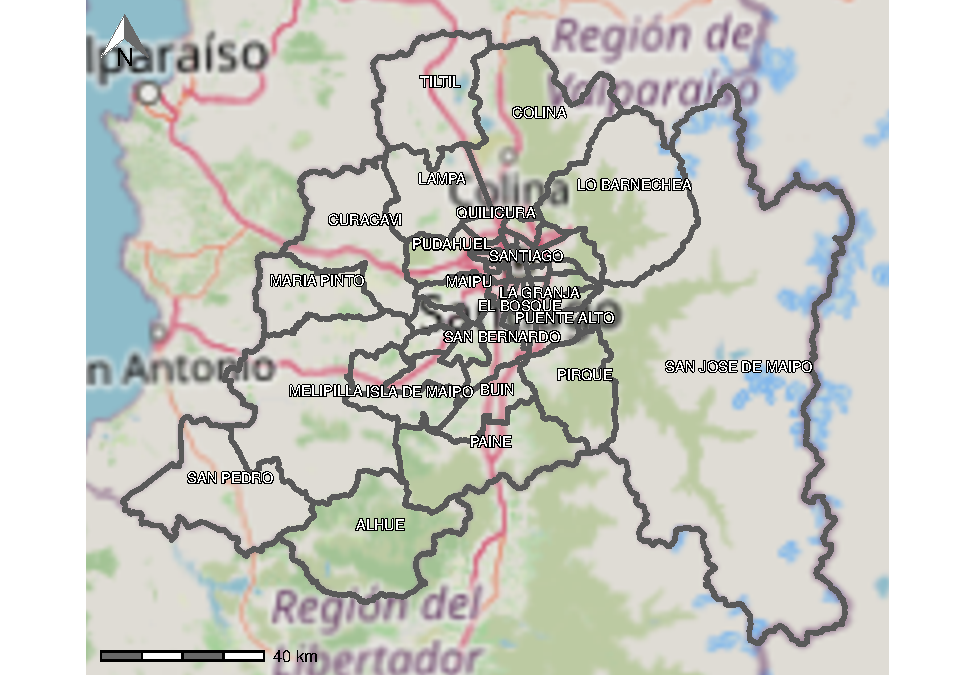
\includegraphics{thesis_files/figure-latex/unnamed-chunk-2-1} 

}

\caption{\label{fig:study boundaries}Santiago the case study}\label{fig:unnamed-chunk-2}
\end{figure}
\hypertarget{descriptive-analysis}{%
\subsection{Descriptive Analysis}\label{descriptive-analysis}}

As mentioned earlier in the study, previous researchers have applied various variables for implementing the ordinal regression model. In this study, we employ a group of dependent and independent variables extracted from individual characteristics and health information parts of the surveys. According to Table \ref{tab:Definitions} for dependent variables, we chose the stress indicator of the level of stress experienced by respondents while commuting and another stress criterion revealing the importance level of stress experienced when travelling by participants. For independent variables, we selected respondents age and income level, occupation, and their primary mode of transportation while regular commuting. As can be seen in the Table \ref{tab:Definitions} there are multiple subcategories for each variable. Furthermore, there would be a regrouping process for the subcategories to reach a more efficient bivariate ordinal model.
\begin{table}

\caption{\label{tab:unnamed-chunk-4}\label{tab:Definitions}Definitions of variables}
\centering
\fontsize{8}{10}\selectfont
\begin{tabular}[t]{l>{\raggedright\arraybackslash}p{10em}>{\raggedright\arraybackslash}p{10em}>{\raggedright\arraybackslash}p{10em}}
\toprule
Name & Note & Variable & Subcategory\\
\midrule
\addlinespace[0.3em]
\multicolumn{4}{l}{\textbf{Socio-Economic and Demographic Attributes}}\\
\hspace{1em}Age & Age of respondents in Santiago in 2016 & NA & {}[Less18], [from18to24years], [from25to34years], [from35to54years], [55to64year], [from65more]\\
\hspace{1em}Income & Level of income of respondents in Santiago in 2016 & NA & {}[Less423], [423to639], [639to977], [977to1550], [1550to2380], [2380more]pesos\\
\hspace{1em}Main\_mode & Main transport mode used by respondents in Santiago in 2016 with eight levels: Car, Taxi, Collective, Motor, Metro, Bus, Bicycle, Walk & NA & Car, Taxi, Collective, Motor, Metro, Bus, Bicycle, Walk\\
\hspace{1em}Education & Level of education of respondents in Santiago in 2016 & NA & Elementary, Secondary, Professor, College, Postgrad\\
\hspace{1em}Occupation & Occupation of respondents in Santiago in 2016 & NA & Full time, Part time, Self employed, Unemployed, Home taker, Student, Student work, Retired, other\\
\addlinespace[0.3em]
\multicolumn{4}{l}{\textbf{Stress Characteristics}}\\
\hspace{1em}Stress & How do respondents assess the level of stress they experience on their usual trips? On Likert scale & NA & Very low feeling of stress, Low feeling of stresS, Moderate feeling of stress, High feeling of stress, Very high feeling of stress\\
\hspace{1em}Importance\_Stress & What is the importance respondents assign to these aspects? On Likert scale & NA & No importance feeling of stress, Slightly important feeling of stress,  Moderately important feeling of stress, Important feeling of stress, Very important feeling of stress\\
\bottomrule
\end{tabular}
\end{table}
To initialize our bivariate ordinal model, we took advantage of previous studies about the importance of different independent variables within individual characteristics as can be seen in Table \ref{tab:Descriptive statistics of variables}.

Although gender looked effective on some of the driver stress scales like confidence and alertness, it was rather weak to indicate gender difference in terms of coping strategies. Previous studies revealed men feel more confident and alert than their counterparts. Regarding coping strategies, women seemed to score higher in cognitive strategies despite men who tend to use behavioural strategies. (Kontogiannis, 2006). Although it has been found that women were more likely to feel stress and anxiety than men, some studies have shown that women and men in rather similar conditions felt the same level of stress (Hill and Ng Boyle, 2007).

Age sounded influential on most aspects of driver stress vulnerability. Getting older had a positive role in a way that it increased cognitive coping strategies useful in decreasing stress levels and declined negative behaviours like aggression (Kontogiannis, 2006), thus they felt less stress.

Another study indicated the relationship of age with stress in a completely different way as some situation-specific tensions tend to increase by getting old until some older ones decide not to drive (Hill \& Boyle, 2007). Age also could be negatively related to the manifestation of violation and dangerous behaviours as old drivers tend to decrease their speed due to declining cognitive capabilities (Westerman \& Haigney, 2000).

In contrast to old people, youth were more likely to reveal their driving anger through behavioural coping strategies(Hill \& Boyle, 2007).

Based on findings of previous research on determinants of an individual's vulnerability to mobility stress, level of education and family status would be influential on the experienced stress while commuting. Also, a high level of income would provide people with the opportunity to purchase a private vehicle limiting their driving stress and uncomfortable experience with public means (Odufuwa, 2008).

In order to achieve a more efficient model, we capitalized on recoding to amalgamate several subcategories within each independent variable into broader categories, thus enhancing the model's efficiency. This approach proves useful in simplifying the model and improving interpretability, particularly in cases where certain subcategories exhibit low frequencies and when our focus lies on identifying higher-level patterns. Furthermore, certain variables, such as the main mode of transportation, have been grouped into new categories, including public, private, and active modes, as opposed to the previous eight categories in Table \ref{tab:Definitions}.
\begin{table}

\caption{\label{tab:unnamed-chunk-5}\label{tab:Descriptive statistics of variables}Descriptive statistics of variables}
\centering
\resizebox{\linewidth}{!}{
\begin{tabular}[t]{lll}
\toprule
Variable & Note & Percentage\\
\midrule
\addlinespace[0.3em]
\multicolumn{3}{l}{\textbf{Socio-Economic and Demographic Attributes}}\\
\hspace{1em}AgeYouth & Age Less18 - 34 years & 57.5 \%\\
\hspace{1em}AgeAdults & Age 35-54 years & 30.3 \%\\
\hspace{1em}AgeSeniors & Age 55 to 65 and more years & 12.2 \%\\
\hspace{1em}IncomeLow Income & Income 423to639 & 31 \%\\
\hspace{1em}IncomeMiddle Income & Income 639to1550 & 35.1 \%\\
\hspace{1em}IncomeHigh Income & Income 1550to2380 more & 33.9 \%\\
\hspace{1em}EducationElementary Education & Education Elementary & 2.3 \%\\
\hspace{1em}EducationHigher Education & Education Secondary to Postgrad & 97.7 \%\\
\hspace{1em}Main\_modePrivate Transportation & Primary Mode Car and Metro & 26.5 \%\\
\hspace{1em}Main\_modePublic Transportation & Primary Mode Taxi, Collective, Metro, Bus & 64.3 \%\\
\hspace{1em}Main\_modeActive Transportation & Primary Mode Bicycle, Walk & 9.3 \%\\
\hspace{1em}OccupationWorking & Occupation Full time, Part time, Self-employed, Student work & 69.5 \%\\
\hspace{1em}OccupationNon Professional & Occupation Unemployed, Home taker, Retired & 7 \%\\
\hspace{1em}OccupationStudent & Occupation Student & 21.7 \%\\
\hspace{1em}OccupationWorkingOther & Occupation Other & 1.8 \%\\
\addlinespace[0.3em]
\multicolumn{3}{l}{\textbf{Stress Characteristics}}\\
\hspace{1em}Stress & Likert scale: Very low feeling of stress & 11.6 \%\\
\hspace{1em}Stress & Likert scale: Low feeling of stress & 23.6 \%\\
\hspace{1em}Stress & Likert scale: Moderate feeling of stress & 32.3 \%\\
\hspace{1em}Stress & Likert scale: High feeling of stress & 20.5 \%\\
\hspace{1em}Stress & Likert scale: Very high feeling of stress & 12 \%\\
\hspace{1em}Importance\_Stress & Likert scale: No importance feeling of stress & 2.5 \%\\
\hspace{1em}Importance\_Stress & Likert scale: Slightly important feeling of stress & 6 \%\\
\hspace{1em}Importance\_Stress & Likert scale: Moderately important feeling of stress & 12.8 \%\\
\hspace{1em}Importance\_Stress & Likert scale: Important feeling of stress & 24.8 \%\\
\hspace{1em}Importance\_Stress & Likert scale: Very important feeling of stress & 53.9 \%\\
\bottomrule
\end{tabular}}
\end{table}
\newpage

Regarding analysis during our bivariate ordinal mode, we reclassified different modes of transportation into three general categories active transportation (walking and cycling), public transportation (taxi, collective, metro and bus) and private transportation (car and motorcycle).

As can be seen (see Figure \ref{fig:Modes of transport}), respondents mostly use public means of transportation with almost 285 out of 451 respondents as their main choice for commuting. Recent studies also have shown that using public transport has formed almost 50\% of motorized trips as a salient example of the popularity of public transportation in Santiago, Chile over the recent years (Pezoa, Basso, Quilodrán, \& Varas, 2023).

Regarding this popularity and to make it more productive, it has been mentioned that public transport in Santiago as a modern and integrated system is called Transantiago referring to a sustainable public transport system for Santiago. By aggregating services such as bus and metro and keeping the fare expenses within a low range, passengers can benefit from an efficient system of transport which was unsuccessful based on Muñoz \& Gschwender (2008) and needs some consideration to work as planners expected.

Following this, the second popular mode of transportation can be assigned to private mode with around 25\% of the whole population or 120 persons. Some users also were interested in eco-friendly modes like walking and cycling with slightly more than 40 people and 10 \% of the whole respondents.
\begin{figure}

{\centering 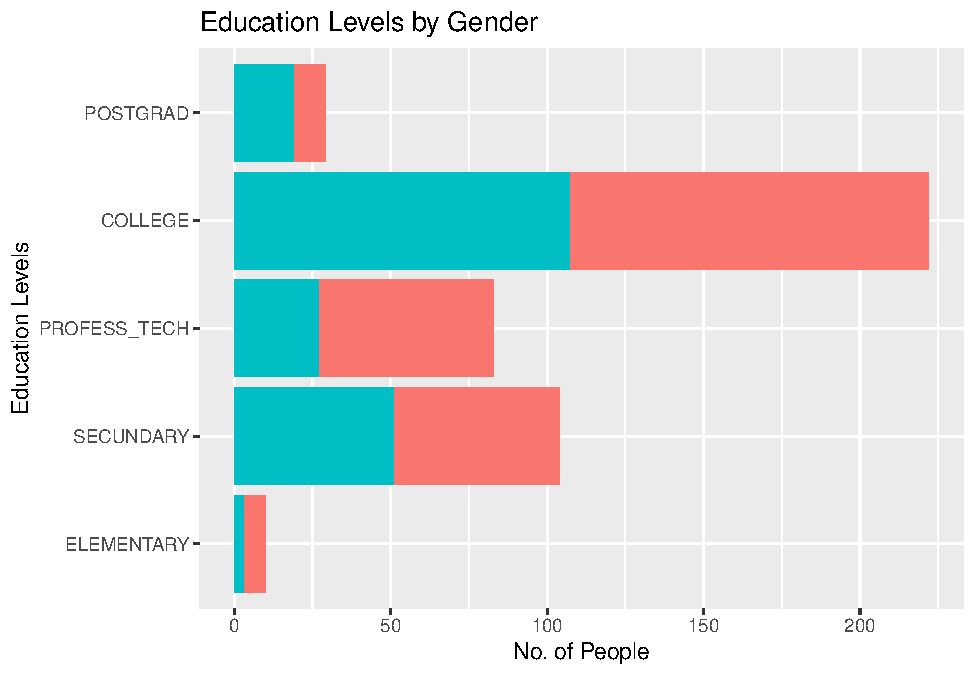
\includegraphics{thesis_files/figure-latex/unnamed-chunk-6-1} 

}

\caption{\label{fig:Modes of transport}Modes of transport}\label{fig:unnamed-chunk-6}
\end{figure}
To have a better understanding of the interaction among the key variables of modes of transportation, age groups, income levels, experienced levels of stress and the importance assigned to the stress, some mosaic plots were adopted.

Mode, age and income are the most crucial variables in our study. As has been studied in previous work, different modes of commuting can be effective on people's feelings and in general, subjective well-being referring to the importance of focusing on individuals' travel experiences such as stress (Smith, 2017).

Income also is one of the significant variables as it determines people's options for commuting. According to the previous research if commuters are low-income workers they tend to use more public transportation in Santiago, Chile (Gómez-Lobo \& Micco, 2023) which is important as it echoes findings of this research about predominance of low and middle income groups in Santiago (see Figure \ref{fig:Income level}) . Another influential variable on people's experience of commuting is age which sometimes makes commuting difficult for older people especially when they choose walking according to the folks in La Cisterna district to the city center in Santiago (Tironi \& Palacios, 2016).
\begin{figure}

{\centering 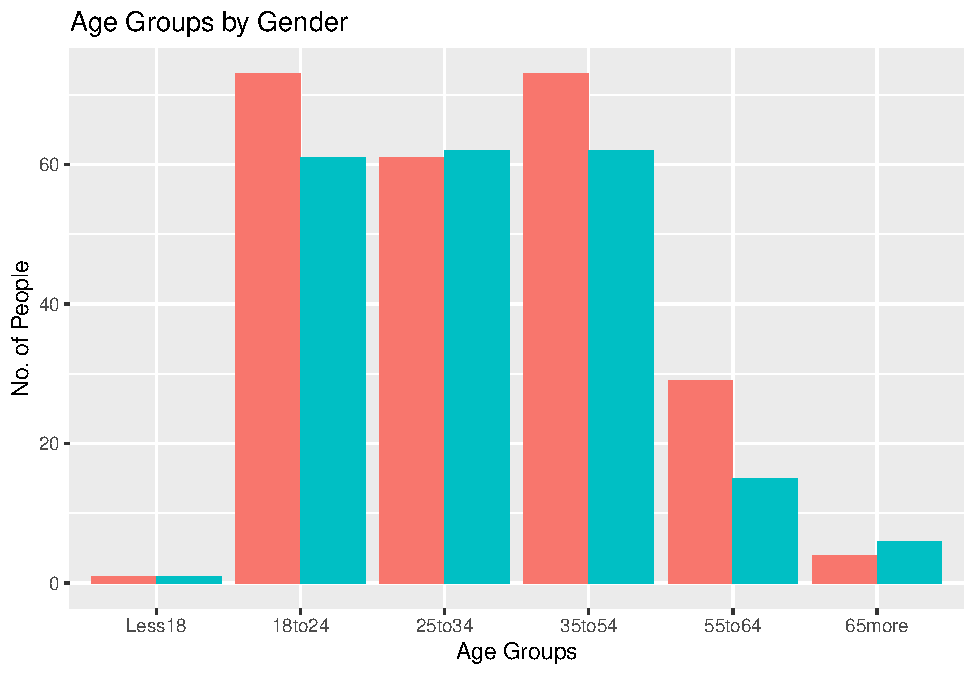
\includegraphics{thesis_files/figure-latex/unnamed-chunk-7-1} 

}

\caption{\label{fig:Income level}Income level}\label{fig:unnamed-chunk-7}
\end{figure}
So we are analyzing these items in terms of their effect on each other.

According to the results from the cross-tabulation of modes of transport by age groups youth as the most populated age group were interested in using active and more public transport with more than 60\% of each. Following this, adults as the second most populated age group were also interested in using more private and afterwards active mode with almost half of the private mode users and 23\% of active mode users, respectively. Apart from this, seniors were mostly interested in private transport with around 15 \% of whole private users and fewer tend to use active and public with about 10 \% for each of them.

Therefore as can be seen (see Figure \ref{fig:Transportation Mode by Age group}) youth respondents tend to use public and active modes, adults are more interested in private and active, and seniors use almost all modes in a similar way but more interested in private mode.
\begin{figure}
\centering
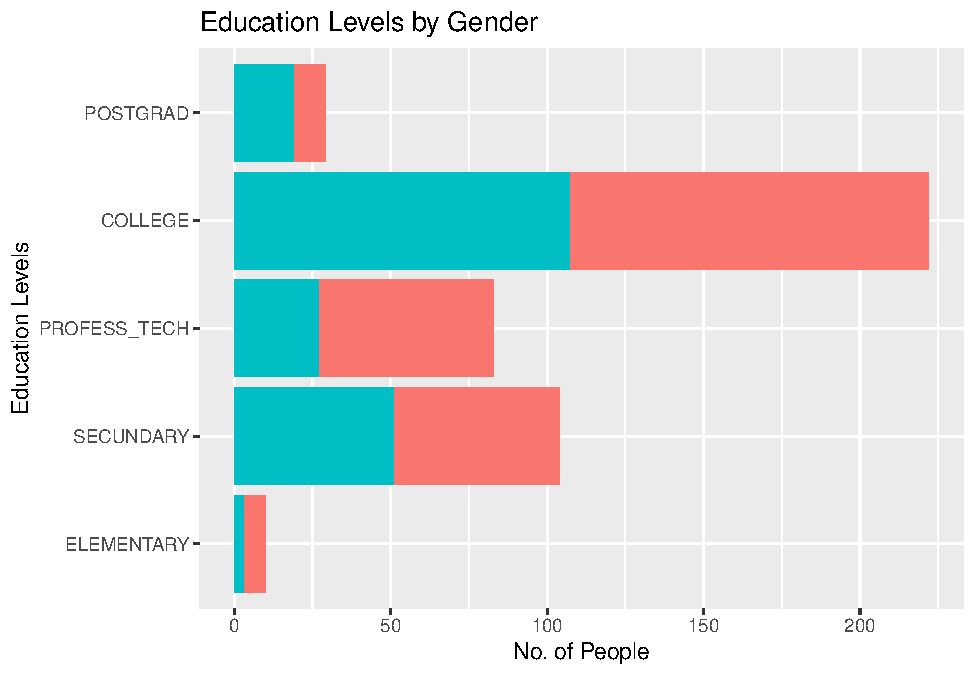
\includegraphics{thesis_files/figure-latex/unnamed-chunk-8-1.pdf}
\caption{\label{fig:unnamed-chunk-8}\label{fig:Transportation Mode by Age group}Transportation Mode by Age group}
\end{figure}
\begin{figure}
\centering
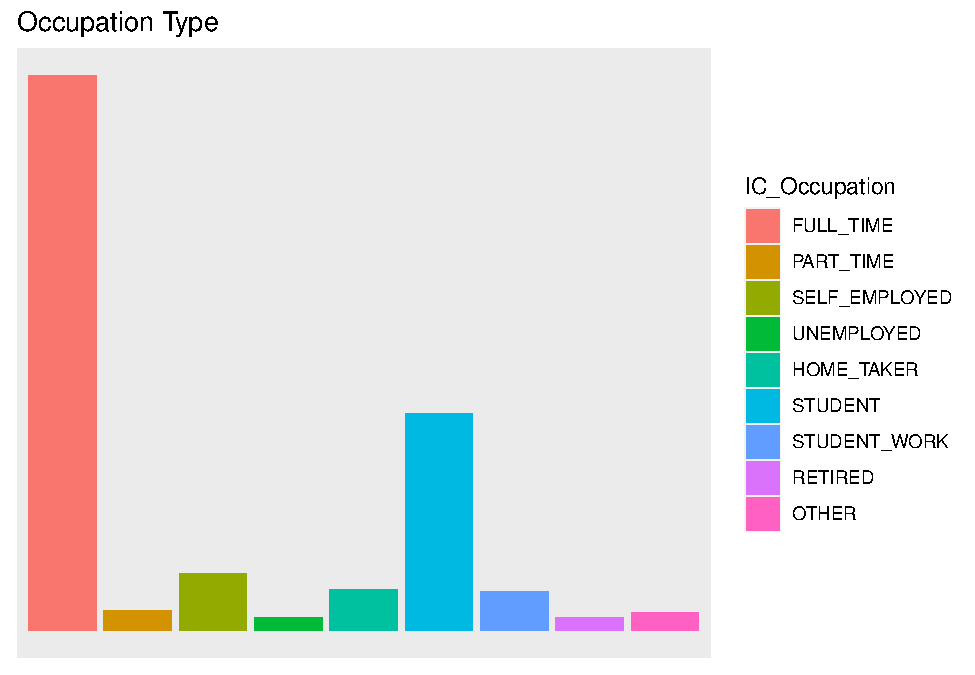
\includegraphics{thesis_files/figure-latex/unnamed-chunk-9-1.pdf}
\caption{\label{fig:unnamed-chunk-9}\label{fig:stress and importance of stress and mode}Conditional Mosaic Plot of Stress Level, Importance of Stress and Mode of Transport}
\end{figure}
As (see Figure \ref{fig:stress and importance of stress and mode}) shows that while active users as the least populated mode of transport, felt mostly low levels of commuting stress, they assigned high importance to that and among all, active users had the highest rate of importance.

To be more in detail, more than 60\% of those who feel very low and low level of stress, give the highest level of importance to that. Following this, an almost opposite trend can be seen for private and public users when they feel high and very high levels of stress, which sounds crucial to them to assign the highest level of importance to their stress feeling.

According to (see Figure \ref{fig:stress and importance of stress and mode}) almost more than 70 \% of public and private users who felt high and very high levels of stress, mentioned that was important to them. Similarly, assigning importance to the rest of these people who felt stress in lower levels slopes to more medium and low levels as the stress level is going to decrease.

It is also an interesting fact that although all users have assigned high levels of importance to stress, private and public transport users felt relatively higher levels of stress compared to their active mode counterparts. Also, these public and private groups comprise almost 90\% of the whole respondents.
\begin{figure}
\centering
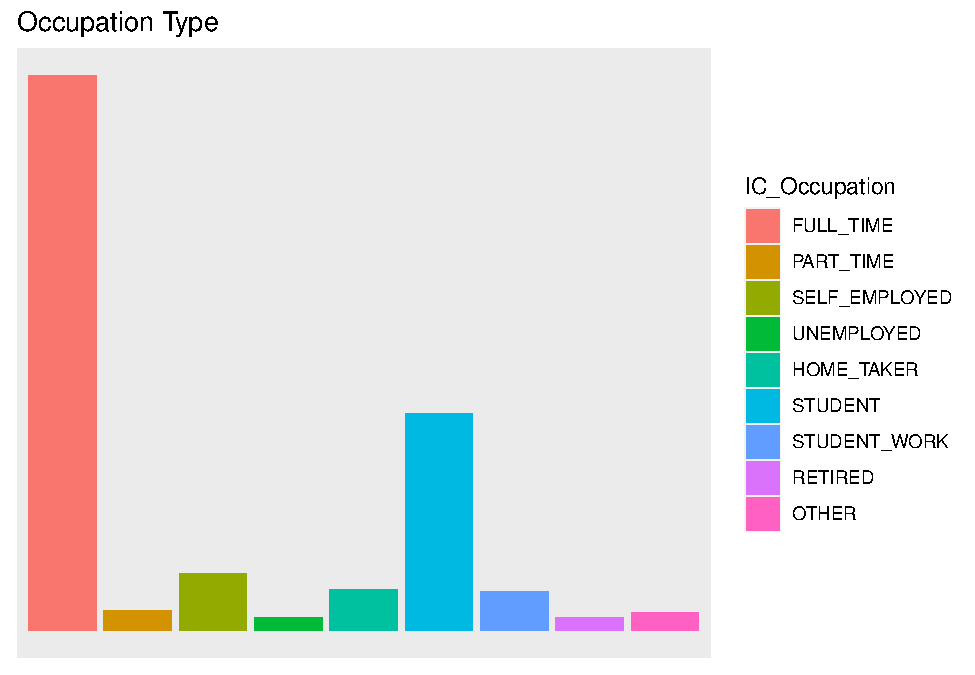
\includegraphics{thesis_files/figure-latex/unnamed-chunk-10-1.pdf}
\caption{\label{fig:unnamed-chunk-10}\label{fig:stress importance of stress and income}Conditional Mosaic Plot of Stress Level, Importance of Stress, and Income Level}
\end{figure}
As (see Figure \ref{fig:stress importance of stress and income}) indicates people in all of the income groups have assigned high levels of importance to stress when commuting. This trend has been indicated from the table (number) that 80 \% of all groups have assigned important and very important levels of feeling stress when commuting. Moreover, the highest rate of giving a high level of importance is associated with the middle-income group all feeling stress levels as the most populated group (almost 33\% of the whole respondents).

It is also interesting that among all of the income groups, low-income users felt the highest level of stress over all of the important stages. On the contrary, a huge number of people belonging to the middle level of income (almost 60 \% of the middle group) felt low and moderate levels of experiencing stress and less than 20 \% of them felt high and very high levels of stress commuting. This can be considered in a similar way for high-income level people as well because the largest part of people felt a range of low to high levels of stress with almost similar percentages to the middle group.

Generally, while almost all people considered high levels of importance about stress, the larger portion of them including middle and high income felt less challenging ranges of stress in comparison to low income levels.
\begin{figure}
\centering
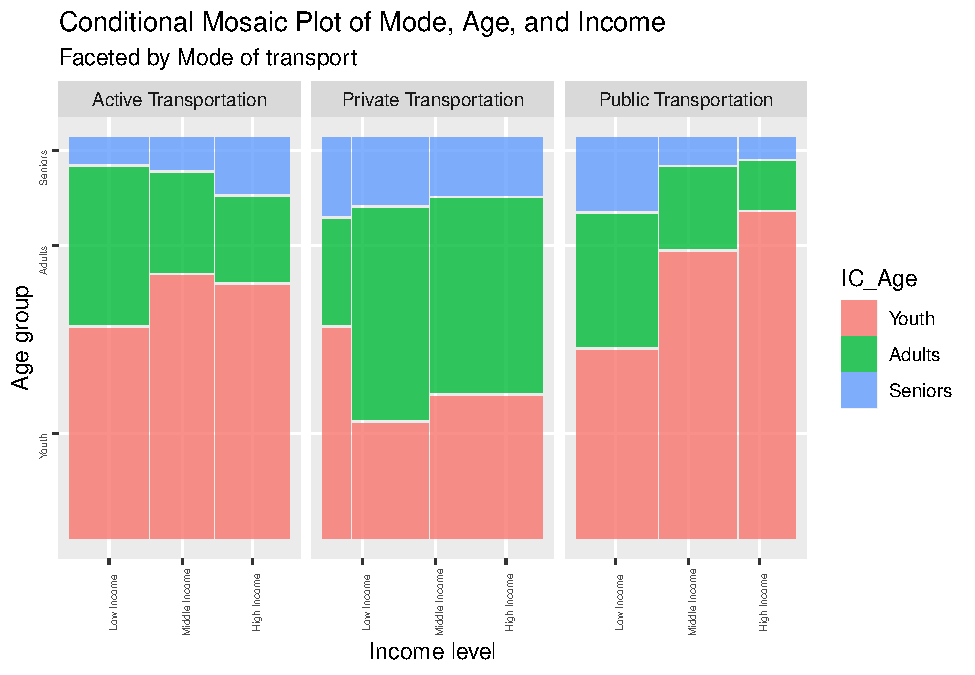
\includegraphics{thesis_files/figure-latex/unnamed-chunk-11-1.pdf}
\caption{\label{fig:unnamed-chunk-11}\label{fig:stress importance of stress and age}Conditional Mosaic Plot of Stress Level and Importance of Stress and Age Groups}
\end{figure}
According to (see Figure \ref{fig:stress importance of stress and age}) youth and adults as the most populated groups incorporate 60\% and 30\% of whole respondents. A common trend among all groups is that around 30\% of them felt moderate stress levels and seniors had the largest portion of feeling stress at a very high level compared to other users.

About youth and adults as the larger portion of respondents, there is a kind of similar dispersion of feeling stress ranging from low to high level with more than 70\% of people in both age groups For the importance of stress, while almost all groups felt a high level of stress, the importance of stress was far more important for adults,and seniors and youth assigned mostly very high level of importance but slightly less than adults.
\begin{figure}
\centering
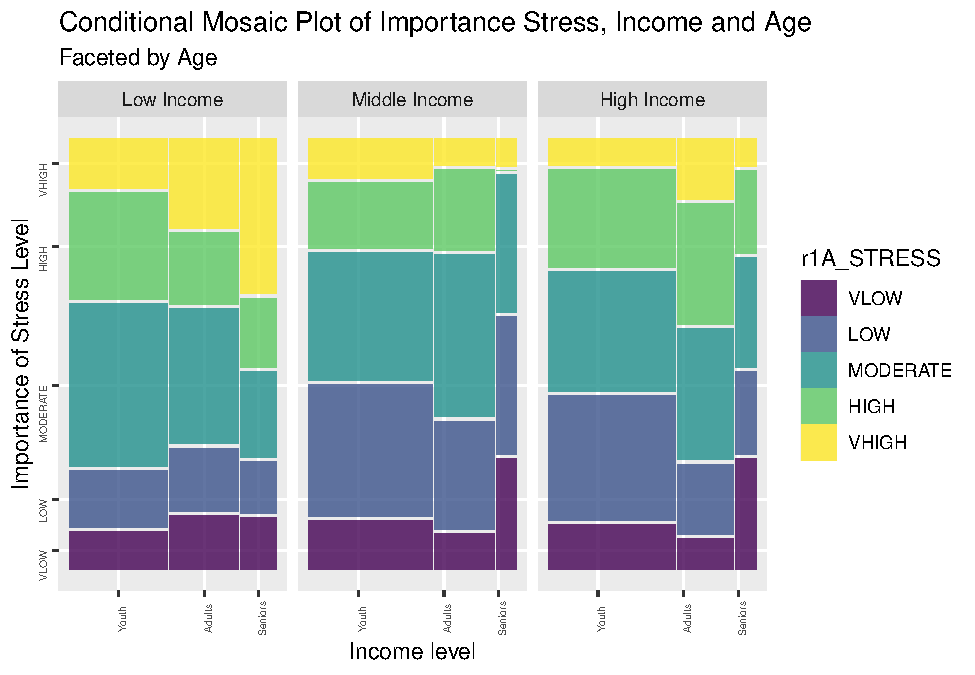
\includegraphics{thesis_files/figure-latex/unnamed-chunk-12-1.pdf}
\caption{\label{fig:unnamed-chunk-12}\label{fig:Income-mode-Age}Conditional Mosaic Plot of Mode, Age and Income}
\end{figure}
The analysis of the data(see Figure \ref{fig:Income-mode-Age}) reveals distinct trends among different age groups in terms of income levels and preferred modes of transportation. The youth category primarily aligns with high-income levels and active transportation modes. In contrast, adults show a notable association with middle income, alongside a relatively minor difference in low income, often opting for private modes of transportation.

Among seniors, there's a prevalence of low-income status, with a preference for private transportation modes. These findings provide insights into the varying preferences and financial considerations that influence transportation choices across age groups.
\begin{figure}
\centering
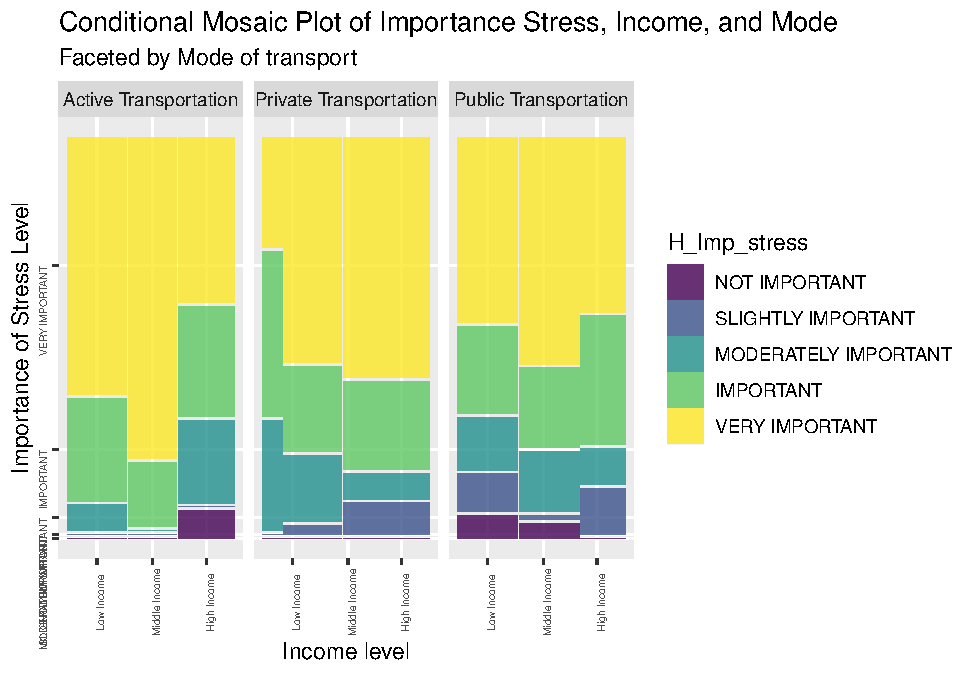
\includegraphics{thesis_files/figure-latex/unnamed-chunk-13-1.pdf}
\caption{\label{fig:unnamed-chunk-13}\label{fig:IMS}Conditional Mosaic Plot of Experienced Stress, Income, Mode}
\end{figure}
As it has been revealed (see Figure \ref{fig:IMS}), almost 80\% of lower-level income people and 65\% of middle-income level as the most populated group use public transport which has been indicated to be highly stressful, especially among low-income ones. High-income respondents where the most interested group in using private mode with 40 \% of them and relatively less commuting stress but they highly rely on public mode with about 50\% among all.
\begin{figure}
\centering
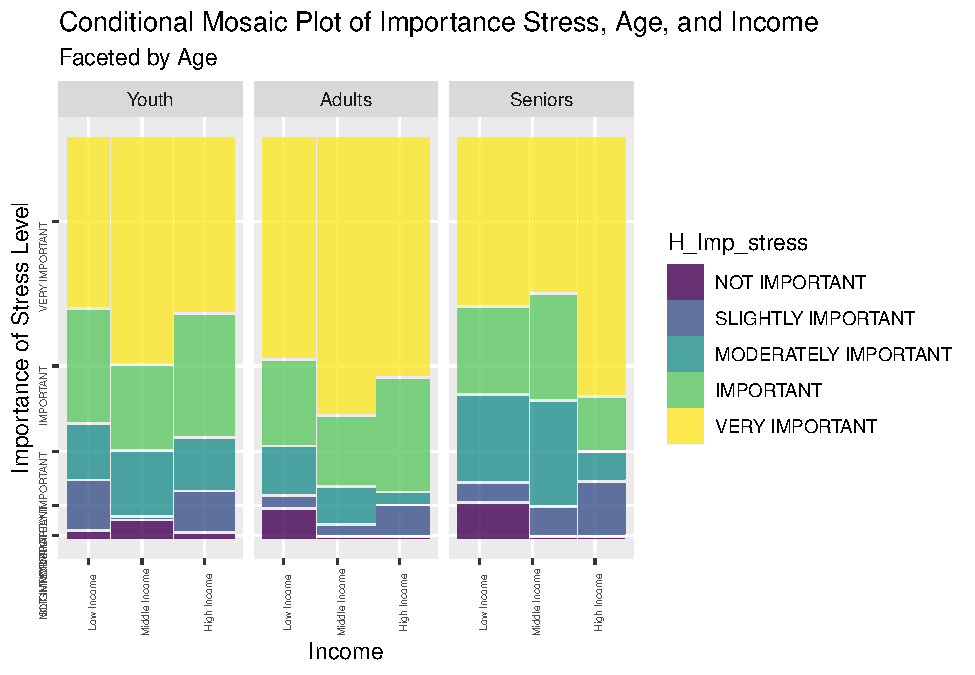
\includegraphics{thesis_files/figure-latex/unnamed-chunk-14-1.pdf}
\caption{\label{fig:unnamed-chunk-14}\label{fig:Income-mode-and-importance-stress}Conditional Mosaic Plot of Importance Stress and Income and Mode}
\end{figure}
The analysis of the provided information reveals (see Figure \ref{fig:Income-mode-and-importance-stress}) distinct patterns within different income groups, stress levels, and transportation modes. Among low-income individuals, the preferred mode of transportation is predominantly public (40.8\%), aligning with a significant prevalence of the ``Moderate'' stress level (37.01\%) and the ``Not important'' stress importance category (37.67\%).

In the middle-income group, ``Active'' transportation is most common (39.2\%), while a majority experiences ``Low'' stress levels (43.2\%). Notably, the ``Very important'' stress category (40.88\%) is prominent. Conversely, high-income individuals tend to favour private transportation modes, coinciding with the highest occurrence of the ``Very high'' stress level (46.3\%). The ``Slightly important'' stress category (75.48\%) also stands out. This comprehensive analysis provides insights into the complex interplay between income, transportation choices, and stress levels and the importance of stress.
\begin{figure}
\centering
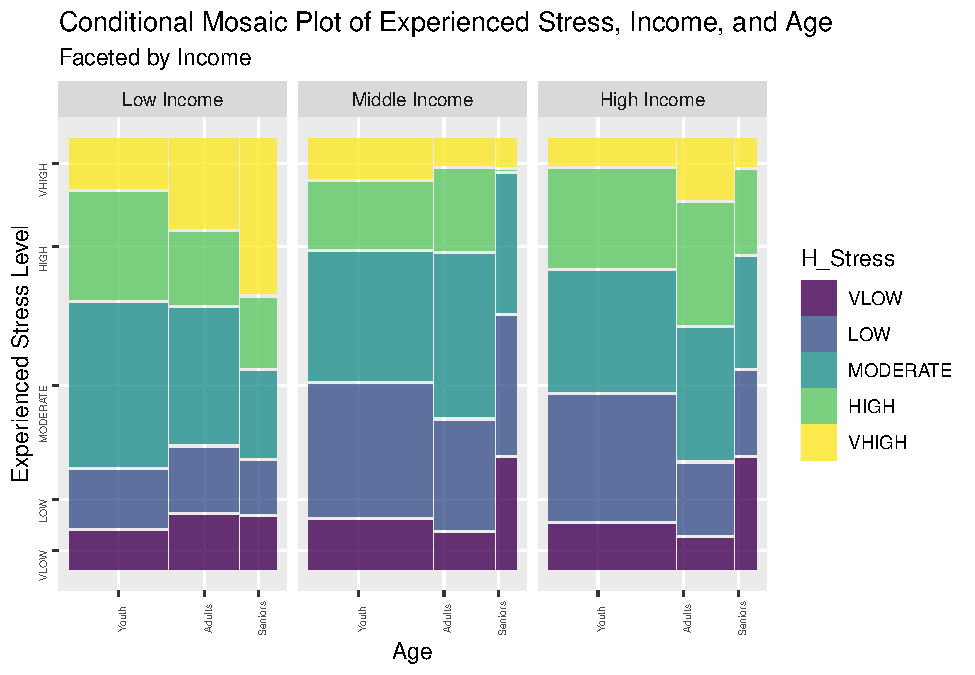
\includegraphics{thesis_files/figure-latex/unnamed-chunk-15-1.pdf}
\caption{\label{fig:unnamed-chunk-15}\label{fig:Income Age and importance of stress}Conditional Mosaic Plot of Importance Stress, Age and Income}
\end{figure}
The analysis of the data (see Figure \ref{fig:Income Age and importance of stress}) categorizes the importance level of stress in association with income and age groups. Middle-income youth, as well as low-income adults and seniors, tend to prioritize stress as ``Not important.'' Meanwhile, stress labelled as ``Slightly important'' is more prevalent among high-income youth, adults, and seniors.

The importance level categorized as ``Moderately important'' can be seen more among middle-income youth, as well as low-income adults and seniors. Among the ``Important'' stress category, high-income youth and adults, along with low-income seniors, stand out. Lastly, the ``Very important'' stress category is mainly linked to middle-income youth and adults, and high-income seniors. This comprehensive breakdown provides valuable insights into how stress perception varies across different income and age groups.
\begin{figure}
\centering
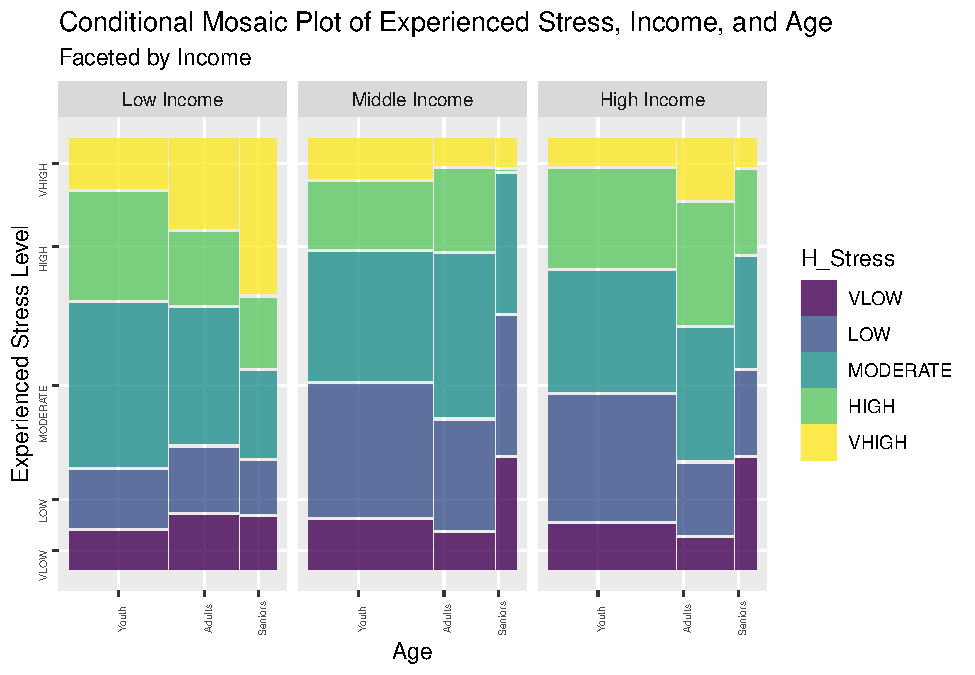
\includegraphics{thesis_files/figure-latex/unnamed-chunk-16-1.pdf}
\caption{\label{fig:unnamed-chunk-16}\label{fig:Income-Age-stress}Conditional Mosaic Plot of Experienced Stress, Income and Age}
\end{figure}
The analysis of the data (see Figure \ref{fig:Income-Age-stress}) presents a segmentation of stress levels based on income and age groups. Stress level categorized as ``Very low'' is highly associated with middle-income youth, low-income adults, and high-income seniors. ``Low'' stress level is prevalent among middle-income youth, adults, and seniors. The ``Moderate'' stress category can be seen more among high-income youth and seniors, as well as low-income adults. Stress level categorized as ``High'' is mainly linked to high-income youth, adults, and seniors. Lastly, the ``Very high'' stress category is primarily related to middle-income youth, low-income adults, and seniors. This comprehensive breakdown offers valuable insights into how stress perception is nuanced across distinct income and age groups.

\hypertarget{modelling-approach}{%
\subsection{Modelling Approach}\label{modelling-approach}}

One of the most common analyses of ordinal data would be related to modelling the preferences or opinions in various fields. In this regard, we can see the application of modelling in correlated ordinal data as multiple outcomes for a number of subjects or objects like participants responding to a questionnaire. Given these multivariate settings, models particularly multivariate ordinal regression models sound practical to deal with the correlation among ordinal outcomes.

The current study has used a similar application of bivariate ordinal regression models (Kenne Pagui \& Canale, 2016) considering the gap between expected satisfaction and experienced service. It refers to two different blocks in that participants are asked to say to what extent the service has importance and in the second part they are required to reveal the actual feeling about the given service.

As can be seen in the study conducted by Hirk, Hornik, \& Gür (2020) the class of multivariate ordinal regression models implemented in mvord and can be applied to other applications such as having multiple or repeated ordinal observations. This research takes advantage of package mvord for R Studio which provides a flexible framework for analysing correlated ordinal data using the class of multivariate ordinal regression models.

This class of modelling assumes each ordinal response as a categorized version of an underlying continuous latent variable separated based on specific threshold parameters. This flexible framework contributes to imposing constraints on thresholds along with regression coefficients using arguments.

In this study, we implement a bivariate logit link for the class of multivariate ordinal regression models. In terms of identifiability, imposing some restrictions on the parameters is needed as the absolute scale and location are not identifiable in ordinal models. Therefore, in order to make the model identifiable, we use one of the options regarding constraining parameters set in the following way:

{[}Fixing the intercept \(\beta_{j0}\) (e.g., to zero), using flexible thresholds \(\theta_j\) and fixing \(\sigma_{ij}\) (e.g., to unity) \(\forall j \in J_i\) and \(forall i \in (1, \cdots, n)\){]}.
(Hirk et al., 2020)

\hypertarget{analysis-and-results}{%
\section{Analysis and Results}\label{analysis-and-results}}

In order to fit our bivariate ordinal regression model, we can use the mvord R package which has two different data structures of MMO and MMO2. As we are working with a wide data format and the covariates stored in different columns of the data set do not change during multiple measurements, using the MMO2 data structure is an appropriate way. In this data structure, each subject i refers to one row of the data frame and all the covariates are stored in different columns.

At this point, we used the following formula to specify the model:

mod\_bivariate \textless- mvord (formula = MMO2(r1A\_STRESS,r1GA\_IMPSTRESS) \textasciitilde{} 0 + r0D\_AGE + r0J\_INCOME + r0P\_MODE1 + r0G\_EDUCATION + r0H\_OCCUPATION ,
link = mvlogit(df = 8L)

Where ``mod\_bivariate'' is the name of the model, ``mvord'' is the function for fitting multivariate ordinal models, and ``MMO2'' is the data structure in accordance with the wide format of the data set. Predicators are demographic variables of the respondents namely their age, income, education and occupation level as well as their primary mode of commute.

The correlation coefficient between H\_Stress and H\_Imp\_stress represents the correlation between the error terms of the two dependent variables. In current study as table (see Table \ref{tab:Bivariate ordered model}) reveals, the estimated correlation coefficient is 0.250344, indicating a positive correlation between the error terms. This positive correlation coefficient suggests that there may be shared or common unobserved factors influencing both stress levels and the importance of stress levels.

Possibly, this phenomenon may be attributed to factors influencing stress levels and the perceived importance of stress that are not captured by the variables included in our model. These unobserved factors could be psychological, environmental, social, or other latent variables that affect individuals' perceptions of stress and its significance. Specifically, the presence of a positive correlation suggests that individuals who experience higher levels of stress may also perceive stress as more important or significant during their commutes.

As the second step to make sure of the model's identifiability and reveal the latent correlation in the model, we used an argument to constrain the coefficients.

\hypertarget{discussion}{%
\section{Discussion}\label{discussion}}

The results of the model analysis can be seen in table (see Table \ref{tab:Bivariate ordered model}). The analysis reveals that adult individuals aged between 35 to 54 are the most affected category when it comes to rating the importance of stress during commuting. There is a positive relation indicating that adults within this age range are more likely to assign importance to stress while commuting.

This trend holds until the age of 54, after which seniors aged 55 and above are significantly related to experiencing stress. The positive coefficient for this age group suggests that their stress level is decreasing compared to their younger counterparts.

This finding may seem incompatible with some previous research claiming that as people get older, they tend to avoid risks and tensions, especially while driving. However, it is important to consider that older individuals may also suffer from cognitive limitations as Westerman \& Haigney (2000) mentioned and have difficulties remembering their lapses, leading to potentially dangerous and stressful situations. This may put them at a higher risk of accidents or unpleasant commuting experiences with more stressful moments. The declining ability to self-monitor and remember specific errors could contribute to this phenomenon (Rabbitt, 1990).

Previous research has indicated that income groups play a significant role in the relationship between travel and satisfaction. It has been suggested that commute satisfaction is associated with commute enjoyment, commute stress, social comparisons, personality, and overall well-being (Ye \& Titheridge, 2019). People with higher incomes are more likely to afford better modes of travel, such as personal drivers, and therefore experience fewer stressful situations.

As can be seen in the model, the higher income category is strongly associated with a negative and relatively large coefficient, even larger than the middle-income group, indicating less probability of experiencing stress. This could be attributed to their capability or overall well-being, enabling them to choose different modes of transportation to avoid stressful commuting experiences. These individuals may utilize problem-solving or emotion-based coping strategies.

As it has been indicated, the more people drive the less stress they experience as they become accustomed to it and this regularity helps them develop coping strategies and become more adept at the drive (Legrain, Eluru, \& El-Geneidy, 2015). Interestingly, the middle-income group, despite having a positive coefficient, does not show a significant association with the experienced stress but it is still positive. However, it is worth noting that this group is highly and positively associated with assigning importance to the experienced stress during commute.

Previous work has also revealed that lower-income groups (which can be considered similar to middle-income) rated instrumental factors (e.g., cost, predictability, flexibility) higher than higher-income groups (Ye \& Titheridge, 2019). This could explain why lower-income (middle-income in our study) individuals are not strongly associated with mentioning the importance of stress. They are more likely to choose public transportation or active modes of transportation due to the limited options available to them.

Moreover, it has been indicated that the impact of commuting mode on stress should be considered by transportation and planning agencies in making decisions (Wener \& Evans, 2011). Commuting specifies the level of perceived control over this process which has a reverse relation with stress (Gottholmseder et al., 2009).

According to the current study, both public and private modes of transportation are positively associated with experiencing stress during commutes. A large coefficient indicates a more significant association between experiencing stress and those who choose public and private modes of transportation than active mode users. These findings are compatible with previous work indicating that commuting by car and public transit is considered to be more stressful and boring than active commuting. This has also been revealed that commuting satisfaction is associated with commute stress to a large extent and hence pedestrians, train travellers, and cyclists are significantly more satisfied with their commuting than car drivers, metro and bus users (Ye \& Titheridge, 2019).

Having a higher level of education has been found to be associated with a positive and relatively significant coefficient leading to a higher probability of assigning importance to self-reported stress while commuting. As already has been mentioned, commute satisfaction has a strong effect on commute stress, and this is followed by the short distance factor(Ye \& Titheridge, 2019). According to a previous study on the effect of telework on daily travel in Sweden, people with higher education are more likely to travel longer and this finding is willing to put travellers more at the exposure of experiencing stress (Elldér, 2020).

In terms of occupation, the current study has shown that experiencing stress among those who have a profession or students is significantly associated. A negative coefficient for both groups implies that their stress level has a decreasing trend compared to their counterparts. In addition, an increasing trend of stress levels has been indicated in some professions like construction due to different reasons like having an unsafe workplace or occupational tensions (Loosemore \& Waters, 2004).

\newpage
\blandscape
\begin{table}

\caption{\label{tab:unnamed-chunk-18}\label{tab:Bivariate ordered model}Estimation Results}
\centering
\resizebox{\linewidth}{!}{
\fontsize{8}{10}\selectfont
\begin{tabular}[t]{lccclccc}
\toprule
Equation1 & beta\_equation1 & se\_equation1 & p\_values\_E1 & Equation2 & beta\_equation2 & se\_equation2 & p\_values\_E2\\
\midrule
- & - & - & - & AgeAdults 1 & 0.5732 & 0.2105 & <0.0001\\
AgeSeniors 1 & -0.5492 & 0.2625 & <0.0001 & - & - & - & -\\
IncomeMiddle Income 1 & -0.9002 & 0.2245 & 1e-04 & - & - & - & -\\
- & - & - & - & IncomeMiddle Income 2 & 0.3625 & 0.2049 & <0.0001\\
IncomeHigh Income 1 & -0.6607 & 0.2248 & <0.0001 & - & - & - & -\\
\addlinespace
Main\_modePrivate Transportation 1 & 1.4984 & 0.3515 & 0 & - & - & - & -\\
Main\_modePublic Transportation 1 & 1.5199 & 0.3175 & 0 & - & - & - & -\\
- & - & - & - & EducationHigher Education 1 & 1.5149 & 0.7432 & <0.0001\\
OccupationWorking 1 & -0.9825 & 0.3217 & 0 & - & - & - & -\\
OccupationStudent 1 & -0.9821 & 0.3677 & <0.0001 & - & - & - & -\\
\addlinespace
VLOW|LOW & -2.275 & 0.4221 & 0 & NOT IMPORTANT|SLIGHTLY IMPORTANT & -1.9388 & 0.7862 & <0.0001\\
LOW|MODERATE & -0.7954 & 0.4246 & <0.0001 & SLIGHTLY IMPORTANT|MODERATELY IMPORTANT & -0.6362 & 0.7312 & <0.0001\\
MODERATE|HIGH & 0.6368 & 0.4283 & <0.0001 & MODERATELY IMPORTANT|IMPORTANT & 0.4615 & 0.7319 & <0.0001\\
HIGH|VHIGH & 1.9855 & 0.4451 & 0 & IMPORTANT|VERY IMPORTANT & 1.6449 & 0.7367 & <0.0001\\
\bottomrule
\end{tabular}}
\end{table}
\elandscape
\newpage

\hypertarget{conclusion}{%
\section{Conclusion}\label{conclusion}}

This study has been conducted to investigate the effect of commuting stress on the transport mode of active and motorized travellers along with coping strategies. Recently, it has been more important in research to evaluate how these consequences are felt by commuters using various modes of transportation, particularly active ones.

Measuring stress entails an individual self-evaluation of a wide variety of variables when commuting preferably while commuting. There is a link between stress and commuting in the literature, which takes into account factors such as time commute as Evans \& Wener (2006) mentioned, control and predictability according to Gottholmseder et al. (2009), as already has been found according to the previous studies about travel motives, especially instrumental ones. The component of stress level has a negative connotation in the context of this research (as no one would prefer to be stressed) and investigates the internal mental reaction of the traveller based on their commuting journeys.

In this research, we aimed to to investigate the perceived commuting stress among active and motorized commuters and the relevant coping strategies. Furthermore, we look into the significance that travellers place on their stress levels. This allows us to investigate the concept of ``limited horizons,'' or how those who are less adaptable normalize subpar experiences. The current study on commuting stress focused on addressing the following questions:

-How crucial it is for respondents to make a journey while feeling a sense of stress and to what scale they are going to evaluate this feeling?

-What elements go into determining how stressed active and motorized travellers are when travelling?

In order to find out how people feel stress while commuting, the association between some key exploratory variables and our income variables has been assessed. The study found that while public users assume the least importance level, they feel the highest level of stress. When we consider a three-way association among active, public and private users, we can see first public and then private users as the more populated groups feel more stress and do not care as much as active users. This result is on the same page with previous work as Brutus, Javadian, \& Panaccio (2017) found those who cycled to work felt less stress than others who commute by motorized modes.

Results also have shown that although public transport is the most popular mode, those who use public transport are mostly low-income. These findings echo results from Tiznado-Aitken, Muñoz, \& Hurtubia (2021), where they found in Latin America due to some deficiencies in land use planning and transport category low-income people suffer from long commutes between work and home. Because of their status and not having a high chance of car ownership, they become captive users of public transport as the fundamental mode of transport.

As previously indicated, low-income people are the most group at the exposure of feeling stress because they are the most interested users of public transport and they do not care about the feeling of stress as much as high and middle-income groups. As Gatersleben \& Uzzell (2007) also supported previous studies people reported more stressful journeys by car and public transit than active mode due to different sources mainly delays because of traffic jams, the behaviour of other (car) users, and poor infrastructure provision (for public users).

It could be also interesting that the least popular mode is active which also has been mostly used by low-income people who are the most careful people about the importance of stress and have undergone the least stress. This echoes similar findings as Smith (2017) has indicated that people who bike and walk to the workplace are happier with their commute experience.

One of the reasons behind this fact that active mode has not been used as the most popular in Chile according to Herrmann-Lunecke, Mora, \& Sagaris (2020) is the lack of physical safety infrastructure (``walkability'' of the sidewalks). Furthermore, the lack of safety in Chile leads to sexual harassment, especially for women making them avoid walking and using public transport and stick to taxis even among those with low budgets.
As expected in Chile as a developing global south country, while high-income clusters are more interested in using public transport, they can be considered as the most users of private modes of transport. These people are the second most affected group by feeling commuting stress and population after low-income people.

Findings have shown that those who use public transport are mostly youth and they feel the highest amount of stress while they assign almost the least importance to their feeling compared to other age groups and modes. Also, people who are dependent on public transport as the most popular mode, which has already been known as the most stressful mode of transport, care about stress less than any other group and they are mostly youth.

Adults are mostly interested in using private transportation and while they feel less commuting stress than public users, they care about it more than them. Seniors as the least populated group are also similar to adults in terms of getting interested in using private transport and they feel the same way as adults. It is interesting to note that active transport users include mostly middle and high-income youth category who don't feel stress that much while commuting but they care about stress more than any other group.

As a study has shown, people associated with low-income levels mostly use public transport feel higher levels of stress while they do not care about that compared to middle-income ones who care about their feeling of stress more than any group. These low-income people are more youth who are more interested in active and public mode at all income levels but their highest experience of feeling stress is when they are using public and the most peaceful is when they use active mode. Although travel could be stressful, there should be a moderator feeling of normalization for them to overcome this stressful experience (Gustafson, 2014).

Moreover, high-income people who are more dependent on private mode feel a very high level of stress and assign a slight rate of importance to their feelings. These people are also more young and adult commuters. The reasons behind why people would stay on their mode of transport choice can be various.

As it has been indicated, respondents in Santiago, Chile are mostly low-income and middle-income. So they probably do not have enough budget to have access to the mode which is less stressful and efficient. Previous findings such as Tironi \& Palacios (2016) support the fact that some commuters despite the anxiety and stress experienced by daily travels using ``Transantiago'' (modern public transportation of Santiago), would decide to sell their private car because of financial issues and stay on public transport. When facing the feeling of stress some people can deal with that or somehow get used to that experience by repeating more and more to develop a sense of ``travel competence'' arising from their attempts to reduce travel-related stress and inconvenience on the road.

While normalization can be beneficial in terms of reducing stress, it could lead to making travel less exciting. In this study we focused mostly on commutes to regular destinations like work, school and so on, we analyzed that these travels come from instrumental motives in which commuters care about their professional goals more than leisure and spare time. For travel to work, people consider factors like environment, cost, health and fitness, convenience and predictability flexibility and obviously, they feel more stress than in recreational travel. So, normalization is going to distinguish between normal travel and fun travel. For fun travel, people tend to commute to longer and unusual trips which seem more exciting whereas for normal travel all activities may become routine and repetitive.

This research demonstrates that the normalization processes possess the capability to moderate and reshape the stressful experiences of travel in various ways. This process can be used as a coping strategy for those who are low-income and have poor access to urban facilities, enough budget and lack of urban fairness in Santiago, Chile.

\hypertarget{conclusion-1}{%
\chapter{Conclusion}\label{conclusion-1}}

Placeholder

\hypertarget{research-contribution}{%
\section{Research Contribution}\label{research-contribution}}

\hypertarget{providing-a-reproducible-data-package-based-on-the-travel-behaviour-of-santiaguinos-commuters.}{%
\subsection{Providing a Reproducible Data Package based on the Travel Behaviour of Santiaguinos Commuters.}\label{providing-a-reproducible-data-package-based-on-the-travel-behaviour-of-santiaguinos-commuters.}}

\hypertarget{influential-attributes-in-commuting-stress-experiences}{%
\subsection{Influential Attributes in Commuting Stress Experiences}\label{influential-attributes-in-commuting-stress-experiences}}

\hypertarget{potential-coping-strategies}{%
\subsection{Potential Coping Strategies}\label{potential-coping-strategies}}

\hypertarget{policy-implications}{%
\section{Policy Implications}\label{policy-implications}}

\hypertarget{invest-in-public-transport-infrastructure}{%
\subsection{Invest in Public Transport Infrastructure}\label{invest-in-public-transport-infrastructure}}

\hypertarget{promote-alternative-transportation-modes}{%
\subsection{Promote Alternative Transportation Modes}\label{promote-alternative-transportation-modes}}

\hypertarget{further-research}{%
\section{Further Research}\label{further-research}}

\hypertarget{exploring-cross-cultural-impacts-on-travel-patterns-and-commuting-stress}{%
\subsection{Exploring Cross-Cultural Impacts on Travel Patterns and Commuting Stress}\label{exploring-cross-cultural-impacts-on-travel-patterns-and-commuting-stress}}

\hypertarget{the-role-of-technology-in-commuting}{%
\subsection{The Role of Technology in Commuting}\label{the-role-of-technology-in-commuting}}

\hypertarget{impacts-of-environmental-factors-on-commuting-experiences}{%
\subsection{Impacts of Environmental Factors on Commuting Experiences}\label{impacts-of-environmental-factors-on-commuting-experiences}}

\hypertarget{study-limitations}{%
\section{Study Limitations}\label{study-limitations}}

\hypertarget{closing-remarks}{%
\section{Closing Remarks}\label{closing-remarks}}

\hypertarget{references}{%
\chapter*{References}\label{references}}
\addcontentsline{toc}{chapter}{References}

Placeholder

\hypertarget{refs}{}
\begin{CSLReferences}{1}{0}
\leavevmode\vadjust pre{\hypertarget{ref-anable2005all}{}}%
Anable, J., \& Gatersleben, B. (2005). All work and no play? The role of instrumental and affective factors in work and leisure journeys by different travel modes. \emph{Transportation Research Part A: Policy and Practice}, \emph{39}(2-3), 163--181.

\leavevmode\vadjust pre{\hypertarget{ref-babore2020psychological}{}}%
Babore, A., Lombardi, L., Viceconti, M. L., Pignataro, S., Marino, V., Crudele, M., \ldots{} Trumello, C. (2020). Psychological effects of the COVID-2019 pandemic: Perceived stress and coping strategies among healthcare professionals. \emph{Psychiatry Research}, \emph{293}, 113366.

\leavevmode\vadjust pre{\hypertarget{ref-benyamini2017normalization}{}}%
Benyamini, Y., Gozlan, M., \& Weissman, A. (2017). Normalization as a strategy for maintaining quality of life while coping with infertility in a pronatalist culture. \emph{International Journal of Behavioral Medicine}, \emph{24}, 871--879.

\leavevmode\vadjust pre{\hypertarget{ref-boran2022psychological}{}}%
Boran, M., Boran, O. F., Korukcu, O., \& Özkaya, M. (2022). The psychological resilience and perceived stress of the frontline heroes in the pandemic in turkey: A descriptive study of the COVID-19 outbreak-mutations-normalization triad. \emph{Japan Journal of Nursing Science}, \emph{19}(1), e12442.

\leavevmode\vadjust pre{\hypertarget{ref-brutus2017cycling}{}}%
Brutus, S., Javadian, R., \& Panaccio, A. J. (2017). Cycling, car, or public transit: A study of stress and mood upon arrival at work. \emph{International Journal of Workplace Health Management}, \emph{10}(1), 13--24.

\leavevmode\vadjust pre{\hypertarget{ref-ellder2020telework}{}}%
Elldér, E. (2020). Telework and daily travel: New evidence from sweden. \emph{Journal of Transport Geography}, \emph{86}, 102777.

\leavevmode\vadjust pre{\hypertarget{ref-evans2006rail}{}}%
Evans, G. W., \& Wener, R. E. (2006). Rail commuting duration and passenger stress. \emph{Health Psychology}, \emph{25}(3), 408.

\leavevmode\vadjust pre{\hypertarget{ref-folkman1985if}{}}%
Folkman, S., \& Lazarus, R. S. (1985). If it changes it must be a process: Study of emotion and coping during three stages of a college examination. \emph{Journal of Personality and Social Psychology}, \emph{48}(1), 150.

\leavevmode\vadjust pre{\hypertarget{ref-gatersleben2007affective}{}}%
Gatersleben, B., \& Uzzell, D. (2007). Affective appraisals of the daily commute: Comparing perceptions of drivers, cyclists, walkers, and users of public transport. \emph{Environment and Behavior}, \emph{39}(3), 416--431.

\leavevmode\vadjust pre{\hypertarget{ref-gomez2023urban}{}}%
Gómez-Lobo, A., \& Micco, A. (2023). Urban commuting time and sick-leave medical license use: An empirical study of santiago, chile. \emph{Economics of Transportation}, \emph{33}, 100287.

\leavevmode\vadjust pre{\hypertarget{ref-gottholmseder2009stress}{}}%
Gottholmseder, G., Nowotny, K., Pruckner, G. J., \& Theurl, E. (2009). Stress perception and commuting. \emph{Health Economics}, \emph{18}(5), 559--576.

\leavevmode\vadjust pre{\hypertarget{ref-gustafson2014business}{}}%
Gustafson, P. (2014). Business travel from the traveller's perspective: Stress, stimulation and normalization. \emph{Mobilities}, \emph{9}(1), 63--83.

\leavevmode\vadjust pre{\hypertarget{ref-herrmann2020persistence}{}}%
Herrmann-Lunecke, M. G., Mora, R., \& Sagaris, L. (2020). Persistence of walking in chile: Lessons for urban sustainability. \emph{Transport Reviews}, \emph{40}(2), 135--159.

\leavevmode\vadjust pre{\hypertarget{ref-hill2007driver}{}}%
Hill, J. D., \& Boyle, L. N. (2007). Driver stress as influenced by driving maneuvers and roadway conditions. \emph{Transportation Research Part F: Traffic Psychology and Behaviour}, \emph{10}(3), 177--186.

\leavevmode\vadjust pre{\hypertarget{ref-hirk2020mvord}{}}%
Hirk, R., Hornik, K., \& Gür, L. V. (2020). Mvord: An r package for fitting multivariate ordinal regression models. \emph{Journal of Statistical Software}, \emph{93}(4), 1--41.

\leavevmode\vadjust pre{\hypertarget{ref-kenne2016pairwise}{}}%
Kenne Pagui, E. C., \& Canale, A. (2016). Pairwise likelihood inference for multivariate ordinal responses with applications to customer satisfaction. \emph{Applied Stochastic Models in Business and Industry}, \emph{32}(2), 273--282.

\leavevmode\vadjust pre{\hypertarget{ref-kontogiannis2006patterns}{}}%
Kontogiannis, T. (2006). Patterns of driver stress and coping strategies in a greek sample and their relationship to aberrant behaviors and traffic accidents. \emph{Accident Analysis \& Prevention}, \emph{38}(5), 913--924.

\leavevmode\vadjust pre{\hypertarget{ref-koslowsky1997commuting}{}}%
Koslowsky, M. (1997). Commuting stress: Problems of definition and variable identification. \emph{Applied Psychology: An International Review}.

\leavevmode\vadjust pre{\hypertarget{ref-koslowsky2013commuting}{}}%
Koslowsky, M., Kluger, A. N., \& Reich, M. (2013). \emph{Commuting stress: Causes, effects, and methods of coping}. Springer Science \& Business Media.

\leavevmode\vadjust pre{\hypertarget{ref-legrain2015stressed}{}}%
Legrain, A., Eluru, N., \& El-Geneidy, A. M. (2015). Am stressed, must travel: The relationship between mode choice and commuting stress. \emph{Transportation Research Part F: Traffic Psychology and Behaviour}, \emph{34}, 141--151.

\leavevmode\vadjust pre{\hypertarget{ref-loosemore2004gender}{}}%
Loosemore, M., \& Waters, T. (2004). Gender differences in occupational stress among professionals in the construction industry. \emph{Journal of Management in Engineering}, \emph{20}(3), 126--132.

\leavevmode\vadjust pre{\hypertarget{ref-maier1976learned}{}}%
Maier, S. F., \& Seligman, M. E. (1976). Learned helplessness: Theory and evidence. \emph{Journal of Experimental Psychology: General}, \emph{105}(1), 3.

\leavevmode\vadjust pre{\hypertarget{ref-mokhtarian2001derived}{}}%
Mokhtarian, P. L., \& Salomon, I. (2001). How derived is the demand for travel? Some conceptual and measurement considerations. \emph{Transportation Research Part A: Policy and Practice}, \emph{35}(8), 695--719.

\leavevmode\vadjust pre{\hypertarget{ref-munoz2008transantiago}{}}%
Muñoz, J. C., \& Gschwender, A. (2008). Transantiago: A tale of two cities. \emph{Research in Transportation Economics}, \emph{22}(1), 45--53.

\leavevmode\vadjust pre{\hypertarget{ref-odufuwa2008gender}{}}%
Odufuwa, B. (2008). Gender differentials, vulnerability and mobility stress coping strategies in nigeria. \emph{Journal of Geography and Regional Planning}, \emph{1}(7), 132.

\leavevmode\vadjust pre{\hypertarget{ref-pezoa2023estimation}{}}%
Pezoa, R., Basso, F., Quilodrán, P., \& Varas, M. (2023). Estimation of trip purposes in public transport during the COVID-19 pandemic: The case of santiago, chile. \emph{Journal of Transport Geography}, \emph{109}, 103594.

\leavevmode\vadjust pre{\hypertarget{ref-rabbitt1990age}{}}%
Rabbitt, P. (1990). Age, IQ and awareness, and recall of errors. \emph{Ergonomics}, \emph{33}(10-11), 1291--1305.

\leavevmode\vadjust pre{\hypertarget{ref-rana2020mental}{}}%
Rana, W., Mukhtar, S., \& Mukhtar, S. (2020). Mental health of medical workers in pakistan during the pandemic COVID-19 outbreak. \emph{Asian Journal of Psychiatry}, \emph{51}, 102080.

\leavevmode\vadjust pre{\hypertarget{ref-shamoa2010aggression}{}}%
Shamoa-Nir, L., \& Koslowsky, M. (2010). Aggression on the road as a function of stress, coping strategies and driver style. \emph{Psychology}, \emph{1}, 35--44.

\leavevmode\vadjust pre{\hypertarget{ref-smith2017commute}{}}%
Smith, O. (2017). Commute well-being differences by mode: Evidence from portland, oregon, USA. \emph{Journal of Transport \& Health}, \emph{4}, 246--254.

\leavevmode\vadjust pre{\hypertarget{ref-tironi2016affects}{}}%
Tironi, M., \& Palacios, R. (2016). Affects and urban infrastructures: Researching users' daily experiences of santiago de chile's transport system. \emph{Emotion, Space and Society}, \emph{21}, 41--49.

\leavevmode\vadjust pre{\hypertarget{ref-tiznado2021public}{}}%
Tiznado-Aitken, I., Muñoz, J. C., \& Hurtubia, R. (2021). Public transport accessibility accounting for level of service and competition for urban opportunities: An equity analysis for education in santiago de chile. \emph{Journal of Transport Geography}, \emph{90}, 102919.

\leavevmode\vadjust pre{\hypertarget{ref-webster2016fight}{}}%
Webster, V., Brough, P., \& Daly, K. (2016). Fight, flight or freeze: Common responses for follower coping with toxic leadership. \emph{Stress and Health}, \emph{32}(4), 346--354.

\leavevmode\vadjust pre{\hypertarget{ref-wener2011comparing}{}}%
Wener, R. E., \& Evans, G. W. (2011). Comparing stress of car and train commuters. \emph{Transportation Research Part F: Traffic Psychology and Behaviour}, \emph{14}(2), 111--116.

\leavevmode\vadjust pre{\hypertarget{ref-westerman2000individual}{}}%
Westerman, S., \& Haigney, D. (2000). Individual differences in driver stress, error and violation. \emph{Personality and Individual Differences}, \emph{29}(5), 981--998.

\leavevmode\vadjust pre{\hypertarget{ref-ye2019determinants}{}}%
Ye, R., \& Titheridge, H. (2019). The determinants of commuting satisfaction in low-income population: A case study of xi???an, china. \emph{Travel Behaviour and Society}, \emph{16}, 272--283.

\end{CSLReferences}
\end{document}
